\documentclass[12pt, english]{article}
\usepackage{graphicx}
\usepackage[colorlinks=true, linkcolor=blue]{hyperref}
\usepackage[hungarian]{babel}
\selectlanguage{hungarian}
\usepackage[utf8]{inputenc}
\usepackage[svgnames]{xcolor}

\usepackage{amsmath}
\usepackage{amsthm}
\usepackage{mathtools}
\usepackage{eucal}
\usepackage{amssymb}
\usepackage{mathrsfs}

\usepackage{tocloft}

\cftsetindents{section}{0em}{3em}
\cftsetindents{subsection}{4em}{3em}
\cftsetindents{subsubsection}{6em}{4em}

\renewcommand\cfttoctitlefont{\hfill\Large\bfseries}
\renewcommand\cftaftertoctitle{\hfill\mbox{}}

\usepackage{listings}
\usepackage{afterpage}
\usepackage[font=small,labelfont=bf]{caption}
\pagestyle{plain}

\definecolor{dkgreen}{rgb}{0,0.6,0}
\definecolor{gray}{rgb}{0.5,0.5,0.5}
\definecolor{mauve}{rgb}{0.58,0,0.82}

\lstset{frame=tb,
language=Python,
aboveskip=4mm,
belowskip=4mm,
showstringspaces=false,
columns=flexible,
numbers=none,
keywordstyle=\color{blue},
numberstyle=\tiny\color{gray},
commentstyle=\color{dkgreen},
stringstyle=\color{mauve},
breaklines=true,
breakatwhitespace=true,
tabsize=3
}

\usepackage{here}
\usepackage{bm}


\textheight=21cm
\textwidth=17cm
\oddsidemargin=-.2cm
\pagestyle{plain}

\usepackage{color}
\usepackage{indentfirst}
\usepackage{ragged2e}

% Expectation symbol
\DeclareMathOperator*{\E}{\mathbb{E}}

\global\let\date\relax
\newcounter{unomenos}
\setcounter{unomenos}{\number\year}
\addtocounter{unomenos}{-1}
\stepcounter{unomenos}
\gdef\@date{ \arabic{unomenos} }

\usepackage[backend=bibtex,style=phys]{biblatex}
\bibliography{references} 

\begin{document}

\begin{titlepage}

\begin{center}
Wginer Fizikai Kutatóközpont \\ Magyar Tudományos Akadémia \\ \@date\\
\vspace*{0.5in}
\rule{150mm}{0.1mm}\\
\vspace*{0.3in}
\begin{Large}
\textbf{Hierarchikus számítások értelmezése \\ a vizuális kortexben\\ mély generatív modellek használatával} \\
\end{Large}
\vspace*{0.3in}
\rule{150mm}{0.1mm}\\
\vspace*{0.4in}
\begin{large}
Alex Olar \\
\end{large}
\vfill
\begin{small}
Témavezetők: \\
\end{small}
\vspace{1mm}
Mihály Bányai, Gergő Orbán \\
\vspace{4mm}

\includegraphics[width=2cm]{logoFAC.png}
\vspace{2mm}
\\ Computational Systems Neuroscience Lab
\end{center}
\end{titlepage}

\newcommand{\CC}{C\nolinebreak\hspace{-.05em}\raisebox{.4ex}{\tiny\bf +}\nolinebreak\hspace{-.10em}\raisebox{.4ex}{\tiny\bf +}}
\def\CC{{C\nolinebreak[4]\hspace{-.05em}\raisebox{.4ex}{\tiny\bf ++}}}

\renewcommand{\thesection}{\Roman{section}}
\renewcommand{\thesubsection}{\Roman{section}. \arabic{subsection}}
\renewcommand{\thesubsubsection}{\Roman{section}. \arabic{subsection}.\arabic{subsection}}

\tableofcontents
\newpage

\section{Bevezetés}

\vspace{7mm}

\subsection{Az elméleti idegtudomány alapjai}

\vspace{7mm}

\par A vizuális kortex egy hierarchikusan felépített egység az emlősök agyában, amelyben az első komputációs réteg (primer vizuális kortex - V1) éleket detektál vizuális stimulusok hatására \cite{hubel1968receptive}. Mivel a vizuális hiearchia végső soron olyan magas szintű reprezentációkért felelős, mint a tárgyak kódolása, így erősen megalapozott azt gondolnunk, hogy a második komputációs réteg a vizuális kéregben (V2) olyan tulajdonságokat von ki a, amelyek az élek kompozíciói, azaz texturák \cite{ZiembaV2}. A V2 beli reprezentációk közel sem olyan alaposan felderítettek, mint a V1 beliek és további felderítése szükséges a mélyek rétegeknek is, melyekről még csekély tudásunk van. Ahhoz, hogy a megértésünket elősegítsük szükségünk van komputációs modellek megalkotására, amelyek képekből tesztelhető predikciókat adnak különböző, mérhető neurális aktivációkra az emlősök agyában \cite{yamins2014performance}. Míg nyilvánvalóan fontos, hogy olyan a modellek változói a valóságban is mérhetőek legyenek, mind emellett szükséges, hogy kellően elabsztrahálják a biofizikai részleteit a neurális csatolásoknak. Ezek miatt az okok miatt a gépi tanulásban kifejlesztett modellek felé fordulunk, hogy ezeket alkalmazva betekintést nyerjünk az emlősök agyában végbemenő számítási modellre. 

\vspace{4mm}

\par Mivel az agy képes generatívan müködni - úgy mint elképzelni dolgokat, amelyek nem létezni, vagy álmodni - így szemelőtt kell tartanunk az ilyen modellek fejlesztését. Ebben a tekintetben a látens reprezentációs modellek bizonyosodtak a legjobb komputációs modelleknek. Ezek közül jelentős a variációs autoenkóder, a mély tanulás egyik aktívan kutatott módszere \cite{kingma2013auto}. Ez a modell magas dimenziós képeket próbal egy alacsony dimenziós vektortérbe beágyazni bizonyos megszorításokkal élve erre a beágyazásra neurális hálók segítségével.

\vspace{4mm}

\par Elméletek sokasága állítja azt, hogy az agy valószínűségi inferenciát csinál, amihez szükséges, hogy az emberek és egyéb állatok tároljanak az agyukban egy világról alkotott modellt. Ez erősen megalapozza a látens kódot tartalmazó modellek felderítését. Mivel a valószínűségi modellekben való tanulás és inferencia általában nem megvalósítható, így a fejlesztett módszerek általában közelítő eljárások.

\vspace{7mm}

\subsection{Motivációk}

\vspace{7mm}

\par A témaválasztást az motiválta, hogy komoly fejlődés érhető el a neurobiológiában a mély tanulási modellek alkalmazásával és fejlesztésével. Sokkal több lényeges információt tudunk ilyen módszerekkel szerezni az emlős agy vizuális kortexének működéséről. Fontos többek között azt is megemlíteni, hogy ez a fajta kutatás interdiszciplináris, hiszen ötvözi a neurobiológiát és az informatikát így komoly kihívást jelent a feladat önmagában is.

\vspace{4mm}

\par Az elmúlt évek beli gyors ütemű fejlődés a gépi tanulásban hasznos eszközöket biztosít arra, hogy vizsgálni lehessen a variációs/probabilisztikus inferenciát, hiszen a variációs autoenkóderek is ezt hajtják végre. Biológia ötletek is segíthetik a fejlesztést, hiszen inspirálódni lehet a vizuális kortex hierarchikus struktúrájából. Célünk, hogy megértsük, hogyan lehet VAE-kkal hierarchikus modelleket építeni és néhány alapvető, de nem triviális tulajdonságát vizsgálunk majd, úgy mint a kontraszt. Ezek a meglátások teszik lehetővé majd a későbbiekben, hogy teljesebb képet kaphassunk az agyi képfeldolgozásról.

\vspace{7mm}

\subsection{Áttekintés}

\vspace{7mm}

\par Az elkövetkező néhány fejezetben bemutatunk néhány különbözp modell amivel a vizuális kortex egyes rétegeit modellezték. Először korai komputációs modellek kerülnek szóva, úgy mint a ritka kódolás \footnote{sparse coding}, mivel ez egy áttörést jelentett a V1 megértésében és leírásában. Errőr áttérünk a jelenlegi mély tanulási modellekre és leírjuk az autoenkóderek, variációs autóenkóderek és létre variációs autoenkóderek működését és a szerepüket abban, hogy jobban megértsük az emlősök vizuális kortexének működését. A VAE és LVAE architektúrák variációs inferenciát hajtanak végre, ez részletesek tárgyalva van matematikailag is. Az elméletről áttérünk majd az modell implementációk részleteire amelyek lehetővé tették a mély neurális hálók tanítását, kiemelve az architektúrák moduláris megvalósítását, amely lehetővé teszi, hogy rengeteg féle különböző komplexitású almodell használatát. A továbbiakban bemutatjuk a használt adathalmazokat és azokat a részleteket amelyeket az analízishez szükségesek. Végül de nem utolsó sorban prezentáljuk az eredményeket, amely során vizsgáljuk adott adathalmaz mellett milyen szerepe van a kontrasztnak különböző adatmanipuláció mellett és, hogy hogyan lehetne ezt független változóként kinyerni a látens kódban. Egy alegység lett annak szentelve, hogy megpróbálja magyarázni, hogy mi szükséges a kontraszt függetlenítéséhez és, hogyan mérhető ez.

\newpage

\section{Számítási modellek}

\vspace{7mm}

\subsection{Korai modellek}

\vspace{5mm}

\par Olshausen és Field voltak az elsők akik előálltak egy olyan modellel \cite{olshausen1996emergence}, amely leírta az első vizuális komputációs réteget. Az alapfelvetésük az volt, hogy egy képnek $I(x, y)$ elő kell állnia lineáris bázisfüggvényekből:


\vspace{4mm}

\begin{equation}
    I(x, y) = \sum_{i}a_i \Phi_{i}(x, y)
\end{equation}

\vspace{4mm}

\par Ahol minden $a_{i}$ páronként dekorrerált $\E (a_i a_j) = \E a_i \E a_j$. Ezek a felvetések három ponthoz voltak szükségesek, így a bázisfüggvényeknek:

\vspace{4mm}

\begin{itemize}
    \item tében lokalizáltnak
    \item orientáltaknak
    \item szürő szerűnek \footnote{különböző skálájú struktúrákra érzékenynek} kellett lenniük
\end{itemize}

\vspace{4mm}

\par A főkomponens analízis \footnote{PCA} nem volt megfelelő erre a feladatra, mert azzal olyan adatot lehet jól leírni, amelyben a komponensek közötti lineáris korrelációk határozzák meg a fő korrelációkat, ellentétben a természetes képekkel ahol magasabb rendű korrelációk a jellemzőek. Ahhoz, hogy ezt elérjék egy olyan módszerrel álltak elő, ami az entrópiát minimalizálja, amellett, hogy ritkán kódolja a természetes képeket. A ritka kódolás alatt azt értették, hogy a bázisfüggvények terének csak egy kisebb alterét használja. A fejlesztett módszer neve ritka kódolás és egy speciális esete az ICA \footnote{Independent Component Analysis - \url{https://redwood.berkeley.edu/wp-content/uploads/2018/08/sparse-coding-ICA.pdf}}.

\vspace{5mm}

\subsection{Variációs autoenkóder - VAE}

\vspace{5mm}

\par Az autoenkódereket általában dimenzióredukciós  módszerként használják, nem felügyelt módszerként. Egy enkóder és egy dekóder struktúrát tartalmaznak amik körülveszik a beágyazott reprezentációt (\ref{fig:auto_encoder_scheme}). .

\vspace{4mm}

\begin{figure}[H]
    \centering
    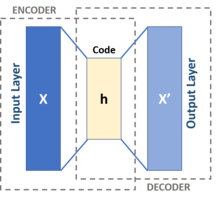
\includegraphics[width=0.3\linewidth]{220px-Autoencoder_schema.png}
    \caption{Egy autoenkóder sematikus ábrája \footnote{\url{https://en.wikipedia.org/wiki/Autoencoder}}}
    \label{fig:auto_encoder_scheme}
\end{figure}

\vspace{4mm}

\par Az autoenkóder modelleket általában neurális hálókként realizálják azok általános függvény approximátor jellege miatt. Fontos eszközei az adattömörítésnek, mivel sokkal jobb eredményeket lehet velük elérni, mint a hagyományos módszerekkel (JPEG) \cite{theis2017lossy}. A variációs autoenkóderek hasonló módon mőködnek amellett, hogy van egy megszorítás a látens kódra. Ez természetesen ront a rekonstrukciós pontosságán magasabb reprezentációs készség reményében.

\vspace{4mm}

\subsubsection{Variációs inferencia autoenkóderekben}

\vspace{4mm}

\par Véve egy adathalmazt $\boldsymbol{X} = \big\{\boldsymbol{\bm{x}}^{(i)}\big\}_{i = 1}^{N}$ ami független és azonosan mintavételezett egy ismeretlen $p(\boldsymbol{X})$ eloszlásból. Feltőtelezhető, hogy az adatnak van egy ismeretlen, nem megfigyelt $\boldsymbol{\bm{z}}$ változója. Feltesszük, hogy ennek értéke $\boldsymbol{\bm{z}}^{(i)}$ egy mintához $\boldsymbol{\bm{x}}^{(i)}$ először egy prior eloszlásból lett véve $p_{\vartheta_{real}}(\boldsymbol{\bm{z}})$ és ezután mintavételezzük $\bm{x}^{(i)}$-t egy feltételes valószínűségi eloszlásból  $p_{\vartheta_{real}}(\boldsymbol{\bm{x}} | \boldsymbol{\bm{z}})$. Mivel a valódi modell paraméterek $\vartheta_{real}$ ismeretlenek, így csak a parametrikus enkóder és dekóder modellekkel közelíthetjük őket. Mivel a poszterior valószínűségeket akarjuk közelíteni:

\vspace{4mm}

\begin{equation}
    p_{\boldsymbol{\vartheta}}(\boldsymbol{\bm{z}} | \boldsymbol{\bm{x}}) \propto p_{\boldsymbol{\vartheta}}(\boldsymbol{\bm{x}} | \boldsymbol{\bm{z}}) p_{\boldsymbol{\vartheta}}(\boldsymbol{\bm{z}})
\end{equation}

\vspace{4mm}

\par Ahol lényegében a Bayes-tételt alkalmaztuk a priorra és a likelihoodra, hogy megkapjuk a poszterior eloszlást \footnote{a valódi poszteriort általános esetben nem lehet kiszámolni, mivel szükség lenne $p_{\vartheta}(\bm{x})$}. Definiálunk egy enkóder/rekogniciós modellt $q_{\phi}(\boldsymbol{\bm{z}} | \boldsymbol{\bm{x}})$ és egy dekóder modellt $p_{\vartheta}(\boldsymbol{\bm{x}} | \boldsymbol{\bm{z}})$. Az enkóder egy valószínűségi eloszlást approximál $\boldsymbol{\bm{z}}$ felett aminek a priorhoz kell hasonlónak lennie, míg a dekóder a valódi eloszlást próbálja közelíteni a mintavételezett látens reprezentáció alapján. Ez egy kétlépcsős generatív folyamat. 

\vspace{4mm}

\par Kingme és Welling cikkében \cite{kingma2013auto} bemutatnak egy olyan variációs modellt ami stochasztikus gradiens módszerrel tanítható, amellett, hogy nem determinisztikus paramétereket is tartalmaz. Ez természetesen nem egyértemű, hiszen a gradiensek propagációja \footnote{back-propagation} sztochasztikus rétegeken keresztül nem megoldott általános esetben. A továbbiakban a módszer leírását prezentáljuk:

\vspace{4mm}

\begin{gather*}
    recognition\ model\ :\  q_{\phi}(\bm{z}|\bm{x}) \xrightarrow{\text{approximates}} p_{\vartheta_{real}}(\bm{z} | \bm{x}) \\
    probabilistic\ decoder\ :\ p_{\vartheta}(\bm{x} | \bm{z}) \xrightarrow{\text{approximates}} p_{\vartheta_{real}}(\bm{x} | \bm{z})
\end{gather*}

\vspace{4mm}

\par Mivel az egyes minták függetlenek $p(\bm{x}^{(1)}, \bm{x}^{(2)}, ..., \bm{x}^{(N)}) = p(\bm{x}^{(1)})p(\bm{x}^{(2)})\cdot ... \cdot p(\bm{x}^{(N)})$ így számolhatunk $p(\bm{x}^{(i)})$-n mindent, közelítőleg $p(\bm{x}^{(i)})$:

\vspace{4mm}

\begin{gather}
    \ln p(\bm{x}^{(i)}) = \ln\int p(\bm{x}^{(i)}, \bm{z})dz \quad from\ marginal\ prob.\ dist.\\
    \ln p(\bm{x}^{(i)}) = \ln\int p(\bm{x}^{(i)}, \bm{z})\frac{q(\bm{z})}{q(\bm{z})}dz \quad introducing\ the\ prior \\
    \ln p(\bm{x}^{(i)}) = \ln \E_{q(\bm{z})} \Big( \frac{p(\bm{x}^{(i)}, \bm{z})}{q(\bm{z})}\Big) \\
    \ln \E_{q(\bm{z})} \Big( \frac{p(\bm{x}^{(i)}, \bm{z})}{q(\bm{z})}\Big) \geq \E_{q(\bm{z})} \ln\Big( \frac{p(\bm{x}^{(i)}, \bm{z})}{q(\bm{z})}\Big) \quad applying\ Jensen's\ inequality \\
    L_{i} = \ln p(\bm{x}^{(i)}) \geq \E_{q(\bm{z})} \ln\Big( \frac{p(\bm{x}^{(i)}, \bm{z})}{q(\bm{z})}\Big) \quad ELBO
\end{gather}

\vspace{4mm}

\par Konvex függvényekre alkalmaztük a Jensen-egyenlőtlenséget. Alkalmazva, hogy $p(\bm{x}, \bm{z}) = p(\bm{x} | \bm{z})p(\bm{z})$ és észrevéve, hogy mi az enkóder/rekogníciós modellt használjuk $q(\bm{z})$ közelítésére $q_{\phi}(\bm{z} | \bm{x})$:

\vspace{4mm}

\begin{equation}
    L_{i} \geq \E_{q_{\phi}(\bm{z} | \bm{x})} \Big( \ln p(\bm{x}^{(i)} | \bm{z}) \Big) + \E_{q_{\phi}(\bm{z} | \bm{x})} \Big( \ln p_{\vartheta}(\bm{z} | \bm{x}^{(i)}) \Big) - \E_{q_{\phi}(\bm{z} | \bm{x})} \Big( \ln q_{\phi}(\bm{z} | \bm{x}^{(i)}) \Big)
\end{equation}

\vspace{4mm}

\par Bevezetjük a Kullback-Leibler-divergenciát ami lényegében két valószínűségi eloszlás között méri a különbséget, így az optimalizációs problémában azt segíti elő, hogy két eloszlás közel kerüljön egymáshoz.

\vspace{4mm}

\begin{gather*}
    KL(q_{\phi}(\bm{z} | \bm{x}^{(i)}) | p_{\vartheta}(\bm{z} | \bm{x}^{(i)})) = \int q_{\phi}(\bm{z} | \bm{x}^{(i)})\ln \frac{q_{\phi}(\bm{z} | \bm{x}^{(i)})}{p_{\vartheta}(\bm{z} | \bm{x}^{(i)})}dz = \E_{q_{\phi}(\bm{z} | \bm{x}^{(i)})} \Big( \ln \frac{q_{\phi}(\bm{z} | \bm{x}^{(i)})}{p_{\vartheta}(\bm{z}|\bm{x}^{(i)})}  \Big) \\ \\
    KL(q_{\phi} | p_{\vartheta}) = -L_{i} + \E_{q_{\phi}(\bm{z} | \bm{x}^{(i)})} \Big( \ln p_{\vartheta}(\bm{x}^{(i)} | \bm{z}) \Big) \quad using\ Bayes-theorem
\end{gather*}

\vspace{4mm}

\par Az algoritmus célja, hogy optimalizálja az ELBO \footnote{variational lower bound} függvényt $\phi, \vartheta$ változókban. Bevezetjük még $p_{\vartheta}(\bm{z} | \bm{x}^{(i)}) \equiv p(\bm{z})$ feltételezett priort minden adatpontra a látensek felett. Mivel az ELBO gradiense $\phi$ változókban problémás és túlzottan számításigényes, így Kingam és Welling megalkották rá a AEVB \footnote{auto-encoding variational Bayes} algoritmust ami lehetővé teszi a gyors gradiens propagációt a neurális hálón keresztül a sztochasztikus réteggel.

\vspace{4mm}

\paragraph{A reparametrizációs trükk \newline \newline}

\vspace{4mm}

\par Legyen $\bm{z}$ a valószínűségi változó amit$   q_{\phi}(\bm{z} | \bm{x})$-ból mintavételeztünk. Bizonyos gyakori esetekben egy ilyen változó kifejezhető \footnote{1. kiszámolható kumulatív eloszlás, 2. norm-scale függvény, 3. függvény kompozíció} egy determiniszitkus függvénnyel $\bm{z} = g_{\phi}(\bm{\epsilon}, \bm{x})$ ahol $\bm{\epsilon}$ egy független valószínűségi változó $p(\bm{\epsilon})$ eloszlással. Mivel valószínűségi eloszlásokra, melyek egymás függvényei $q_{\phi}(\bm{z} | \bm{x})|d\bm{z}| = p(\bm{\epsilon})|d\bm{\epsilon}|$, így $f(\bm{z})$ várható értéke:

\vspace{4mm}

\begin{equation}
    \int f(\bm{z})q_{\phi}(\bm{z} | \bm{x}^{(i)})d\bm{z} = \int p(\bm{\epsilon})f(g_{\phi}(\bm{\epsilon}, \bm{x}^{(i)})) d\bm{\epsilon} \approx \frac{1}{L}\sum_{l=1}^{L}f(g_{\phi}(\bm{\epsilon}^{(l)}, \bm{x}^{(i)}))
\end{equation}

\vspace{4mm}

\par Ahol $\bm{\epsilon}^{(l)}$-t $p(\bm{\epsilon})$-ből mintavételeztük. Ha $q_{\phi}(\bm{z} | \bm{x})$ normál eloszlás $\bm{z} \sim N(\bm{\mu}, \bm{\sigma})$ akkor egy evidens reparametrizáció $g_{\phi}$ a következő alakban írandó $\bm{z} = \bm{\mu} + \bm{\epsilon} \odot \bm{\sigma}$.

\vspace{4mm}

\begin{figure}[H]
    \centering
    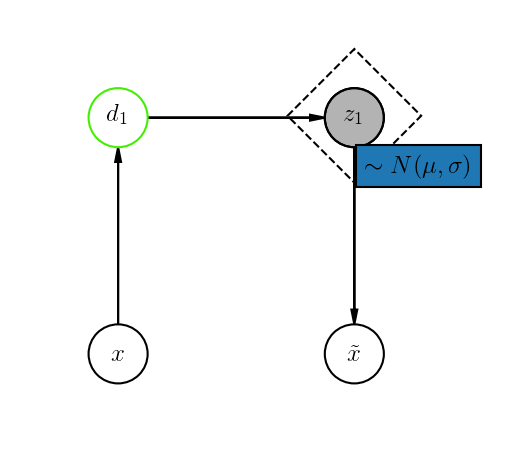
\includegraphics[width=0.33\linewidth]{vae.png}
    \caption{Variációs autoenkóder}
    \label{fig:vae}
\end{figure}

\vspace{4mm}

\par A (\ref{fig:vae}) ábrán a variációs autoenkóder látható. Az egyik neurális haló közelíti $q_{\phi}(\bm{z} | \bm{x})$ eloszlást az adathalmazt látva és feltételezzük, hogy többváltozós Gauss eloszlást vesz fel mint a valós, nem kiszámolható poszterior $p_{\vartheta_{real}}(\bm{z} | \bm{x})$.

\vspace{4mm}

\par Mintavételezzük $\bm{z}$-t egy normál eloszlásból ahol az átlag és a szórás a probabilisztikus enkóder modell kimenete. Ezután alkalmazzuk rá a reparametrizációs trükköt. Ezáltal az ELBO függvény egyszerűvé válik:

\vspace{4mm}

\begin{equation}
    L_{i} \simeq \frac{1}{2}\sum_{j = 1}^{J}\Big( 1 + \ln(\sigma^{(i)}_{j})^{2} - (\mu^{(i)}_{j})^{2} - (\sigma^{(i)}_{j})^{2} \Big) + \frac{1}{L}\sum_{l=1}^{L}\ln p_{\theta}(\bm{x}^{(i)} | \bm{z}^{(i, l)})
    \label{eq:ELBO}
\end{equation}

\vspace{4mm}

\par Ahol $\bm{z}^{(i, l)} = \bm{\mu}^{(i)} + \bm{\sigma}^{(i)} \odot \bm{\epsilon}^{(l)}$ és $\bm{\mu}, \bm{\sigma}$-t $q_{\phi}(\bm{z} | \bm{x})$ eloszlásból, míg $\bm{\epsilon}$-t $p(\bm{\epsilon}) \sim N(0, 1)$ eloszlásból vételeztük. Az első tag az egyenletben a Kullback-Leibler-divergencia egy normáls eloszlás és egy egység normál eloszlás között, ami analitikusan számolható és behelyttesítettük \ref{eq:ELBO}-be.

\vspace{4mm}

\par A gyakorlatban ez azt jelenti, hogy a KL-tag könnyen és gyorsan számolható a beagyazás után. Ahhoz, hogy a tanító folyamatot felgyorsuljon és ne kelljen többször átadni a dekóder modellnek a reparametrizált tagot így $L = 1$ a szokásos választás. Folytonos pixelértékek esetén az ELBO függvény második tagja egy többdimenziós Gauss-függvénnyel közelíthető, míg bináris pixelértékek esetén egy Bernoulli-eloszlással.

\vspace{5mm}

\subsection{Létra variációs autoenkóder - LVAE}

\vspace{5mm}

\par A létra variációs autoenkódert 2016-ban fejleszették \cite{sonderby2016ladder} egy évvel az orvosi alkalmazásokban híres UNET \cite{ronneberger2015u} architektúra után, amely hasonló létra szerű kapcsolatokat használ a tanítás során az információ átadására. A létra szerű modellek 2015 után futottak fel a mély tanulás sok területén.

\vspace{4mm}

\par Az LVAE modell lényegileg csak az enkóder modellben különbözik $q_{\phi} (z | x)$ a variációs autoenkódertől azáltal, hogy több sztochasztikus réteget vezet be, hogy pontosabb rekonstrukciókat érjen el és, hogy a mélyebb rétegek által egy magasabb szintű reprezentációt produkáljon. A \cite{sonderby2016ladder} cikkben a valós poszterior eloszlást $p_{\theta_{real}}$  úgy közelítették, hogy szétszedték azt L rétegre:

\vspace{4mm}

\begin{equation}
    p_{\theta_{real}}(\bm{z}) =  p_{\theta}(\bm{z}_{L})\prod_{i = 1}^{L - 1}p_{\theta}(\bm{z}_i | \bm{z}_{i+1})
\end{equation}

\vspace{4mm}

\par A gyakorlatban egy réteget adtunk a variációs autoenkóderhez, ahogy ezt a fentebb említett cikkben is tették. Itt:

\vspace{4mm}

\begin{gather*}
    p_{\theta}(\bm{z}_L) = N(\bm{z}_L  ~ | ~ 0, 1) \quad called\ \epsilon\ previously\\
    p_{\theta}(\bm{z}_i ~ | ~ \bm{z}_{i+1}) = N(\bm{z}_i ~ |  ~ \mu_{p,i}(\bm{z}_{i+1}), \sigma_{p, i}(\bm{z}_{i+1}))
\end{gather*}

\vspace{4mm}

\par Természetesen az itt kijelölt eset folytonos pixel-értékekre igaz. Bináris pixel értékek eseten a második eloszlás Bernoulli alakot vesz fel.

\vspace{4mm}

\begin{figure}[H]
    \centering
    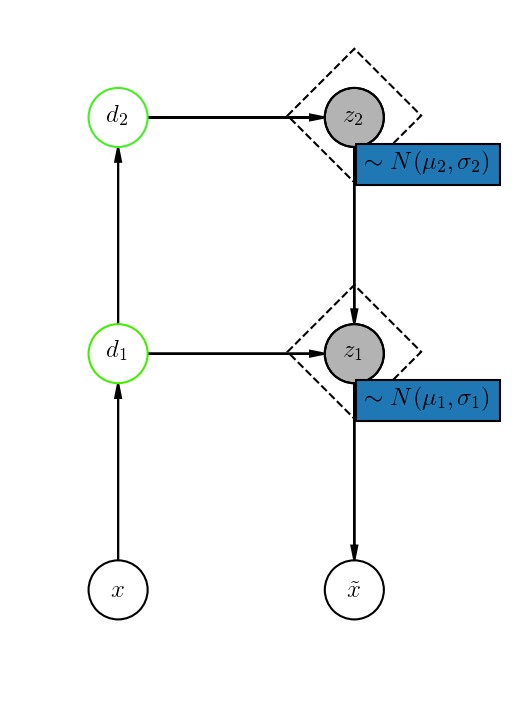
\includegraphics[width=0.35\linewidth]{lvae.png}
    \caption{Létra variációs autoenkóder}
\end{figure}

\newpage

\section{Használt képi adathalmazok}

\vspace{7mm}

\par Főkent szintetikusan generált textura családokat használtnunk a modellek kiértékelése során \footnote{\url{www.rmki.kfki.hu/~banmi/textures/}} amelyek hasonlítanak a  Simonchelli-Portilla textúra családokra \cite{portilla2003image}, de néhány kisérletet végeztünk az MNIST, Fashion-MNIST \cite{xiao2017fashion}, CIFAR-10 és dSprites adathalmazokon \cite{matthey2017dsprites} is. A kísérletek célja volt kideríteni, hogy függetleníteni lehet-e a kontrasztot a látens paraméterekben a tanult képi adatok alapján.

\vspace{4mm}

\par A szintetikus textura család hét különböző textúra fajtát tartalmaz. Az implementációban globális kontraszt normalizációt használtunk, amely megkeresi az adott osztályok középértéket, eltávolítja, majd az osztályokhoz tartozó szórásokat is kiegyenlíti. Ezáltal biztosítható, hogy az osztályok között ne legyen globális kontraszt imbalansz. Ezen felül tanítási időben manipulálni lehet az egyes képeket extra kontraszttal, hogy az egyes struktúrák könnyebben vagy nehezebben felismerhetőek legyenek.

\vspace{4mm}

\begin{figure}[H] 
  \label{fig:texture-families} 
  \begin{minipage}{0.48\linewidth}
    \centering
    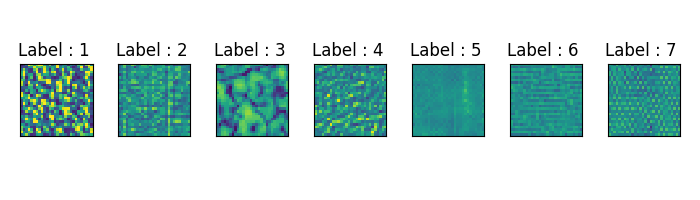
\includegraphics[width=.95\linewidth]{default.png} 
    \caption{Textúra családok} 
  \end{minipage}
  \begin{minipage}{0.48\linewidth}
    \centering
    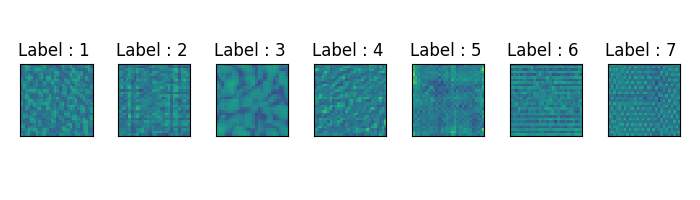
\includegraphics[width=.95\linewidth]{normalized.png} 
    \caption{Normalizált textúra családok} 
  \end{minipage} 
  
  
  \begin{minipage}{0.48\linewidth}
    \centering
    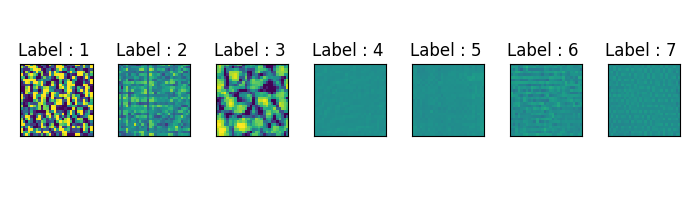
\includegraphics[width=.95\linewidth]{default_contrast.png} 
    \caption{Textúra családok - extra kontraszt} 
  \end{minipage}%% 
  \begin{minipage}{0.48\linewidth}
    \centering
    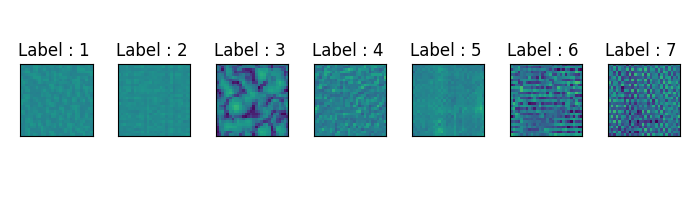
\includegraphics[width=.95\linewidth]{normalized_contrast.png} 
    \caption{Normalizált textúra családok - extra kontraszt} 
  \end{minipage} 
\end{figure}

\newpage

\section{Implementációs részletek}

\vspace{7mm}

\par Főként $\beta-$VAE és ($\beta-$)LVAE architektúrákat használtunk, a korábban levezett célfüggvénnyel, amiben a $\beta$ változó értéke állítja be a Kullback-Leibler-divergencia erősségét:

\vspace{4mm}

\begin{equation}
    L_{i} \simeq \beta_{max}\frac{1}{2}\sum_{j = 1}^{J}\Big( 1 + \ln(\sigma^{(i)}_{j})^{2} - (\mu^{(i)}_{j})^{2} - (\sigma^{(i)}_{j})^{2} \Big) + \frac{1}{L}\sum_{l=1}^{L}\ln p_{\theta}(\bm{x}^{(i)} | \bm{z}^{(i, l)})
\end{equation}

\vspace{5mm}

\subsection{Architektúrális áttekintés}

\vspace{5mm}

\par A modelleket Kerasban \cite{chollet2015keras} implementáltuk és a beépített vizualizációs eszközét használva az implementációs gráf sematikus rajza kinyerhető:

\vspace{4mm}

\begin{figure}[H]
    \centering
    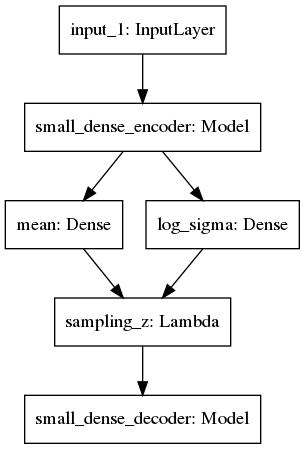
\includegraphics[width=0.25\textwidth]{vae_keras.png}
    \caption{Variációs autoenkóder implementáció - Keras}
\end{figure}

\vspace{4mm}

\par Egy kicsit zavaró lehet, hogy a grafikus modellekkel ellentétben itt a nyilak paraméterátadásokat jelentenek, míg a gráf pontjai almodelljei a gráfnak és nem valószínűségi változók. Tovább lépve az LVAE implementációra:

\vspace{4mm}

\begin{figure}[H]
    \centering
    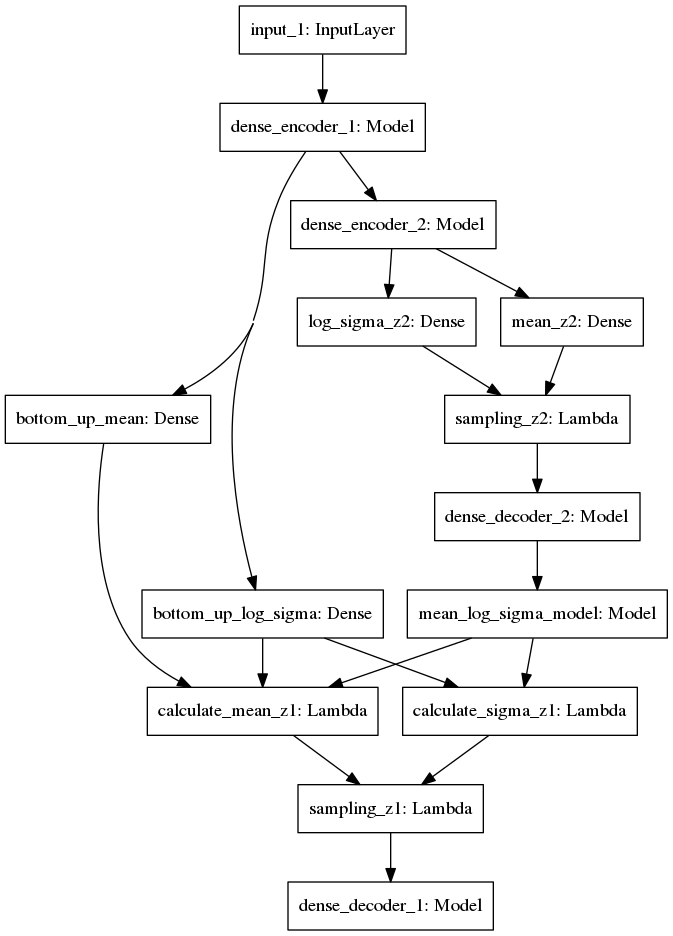
\includegraphics[width=0.6\linewidth]{dense_lvae_keras.png}
    \caption{Létra variaációs autoenkóder implementáció - Keras}
    \label{fig:keras_lvae}
\end{figure}

\vspace{4mm}

\par A Keras segítségével magas szintű modularitás volt eléhető, így az előbbi két ábrán látható `Model` feliratú blokkok szabaton cserélhetőek akármilyen gépi tanulásban használt architektrúrára. 

\vspace{5mm}

\subsection{Növekvő $\beta$-tanulás}

\vspace{5mm}

\par Az LVAE cikkből \cite{sonderby2016ladder} átvéve mi is használtuk a növekvő $\beta$ tanulást, ami alatt azt kell érteni, hogy az összes iteráció 3/7-éig inkrementálisan növelve volt a $\beta$ értéke $\beta = \beta_{max}$-ig, ezután a maximális értekkel tovább folyt a tanítás, hogy konvergáljon a modell. A $\beta_{max}$ érték a tanítás elkezdése előtt függvény paraméterként megadható is direkt módon hatással van a tanulásra, hiszen a KL-tagot befolyásolja.

\vspace{4mm}

\par A VAE és LVAE modellek mindegyékében használva van a reparametrizációs trükk a legmélyebb szotachasztikus rétegen, hogy később mintavételezéskor egy egység szórású, nulla közepú normál eloszlásbol lehessen mintavételezni:

\vspace{4mm}

\begin{equation}
    \boldsymbol{\bm{z}}^{(i, l)} = \boldsymbol{\mu}^{(i)} + \boldsymbol{\sigma}^{(i)} \odot \boldsymbol{\bm{\epsilon}}^{(l)}
\end{equation}

\vspace{4mm}

\par Ahol $\boldsymbol{\bm{\epsilon}}^{(l)} \sim \boldsymbol{N}(0, 1)$. Ahhoz, hogy generatív irányban használjuk a modelljeinket csak ebből a prior eloszlásból kell mintavételeznünk és átadnunk a dekóder modellnek, hogy új, addig nem látott mintákat generálhasson a közelítőleg megtanult $p_{\vartheta_{real}}(x | z)$ eloszlásból.

\vspace{5mm}

\subsection{Generatív modell mintavételezés}

\vspace{5mm}

\par Mindkét modellben (VAE, LVAE) lehetséges tanítás után a mintavételezés. Míg ez a VAE esetében egyértelmű \footnote{random vektor mintavételezése $\p(\epsilon)$-ból, majd dekódolás} ellenben az LVAE esetén a dekóder modellben a bemeneti képből származó információ is jelen van, mivel a második sztochasztikus réteg átlaga és szórása a legmélyebb sztaochasztikus rétegből és a bemeneti képből származtatható. Ezeket bottom up - $\bm{bu}$ és top down $\bm{td}$ komponenseknek nevezzük és generatív irányban a $\bm{bu}$ tag nincs jelen. Nem generatív irányban, a tanítás során determiniszitkusan számolandó:

\vspace{4mm}

\begin{gather}
    \label{eq:z1-mean-sigma-1}
    \hat{\sigma}_{1} = \frac{1}{\sigma_{bu}^{-2} + \sigma_{td}^{-2}} \\
    \hat{\mu}_{1} = \frac{\mu_{bu}\sigma_{bu}^{-2} + \mu_{td}\sigma_{td}^{-2}}{\sigma_{bu}^{-2} + \sigma_{td}^{-2}}
    \label{eq:z1-mean-sigma-2}
\end{gather}

\vspace{4mm}

\par Amikor mintavételezzük $\bm{z}^{(2)}$-t, a legmélyebb sztochasztikus réteg látens vektorához akkor a $\bm{bu}$ szórást végtelennek tekintjük, ezáltal generatív irányben az LVAE paraméterei leegyszerűsödnek:

\vspace{4mm}

\begin{equation}
    \hat{\sigma}_{1} = \sigma_{td}^{2} \quad \quad \hat{\mu_{1}} = \mu_{td}
    \label{eq:ladder-vae-sampling}
\end{equation}

\vspace{4mm}

\par Ez lehetővé teszi azt, hogy ellenőrizzük a tanított modellt. Egy teljes rekonstrukció során össze tudjuk hasonlítani a $\bm{td}$ és a $\bm{bu}$ komponenseket a tényleges szórás és átlag paraméterekkel amiket a rendszer tanul. Ha a $\bm{bu}$ csak zajt tesz a rekonstrukciókra, azaz a szórása és átlaga is nagyon eltér, akkor lényegileg nem kaptunk hierarchikus reprezentációt, míg ha kellően hasonló, generatív irányban is megfelelően tud működni. Ezt egy kősbbi szekcióban tárgyaljuk.

\vspace{4mm}

\par Az implementáció főként `dense` rétegeket \footnote{lényegében mátrix szorzás és eltolás} valamint ReLU \footnote{rectified linear unit} aktivációkat használ a különböző modellekben. Lényegében a két egységből álló enkóder és dekóder modellek az LVAE implementációban úgynevezett MLP \footnote{multilayer perceptron} almodellek, ugyan ez elmondható az egy egységes VAE implementációkról. Néhol ReLU helyett PReLU \footnote{parametric rectified linear unit} aktivációk vannak. Nem csak variációs modelljeink vannak, mivel a megfelelő összehasonlítás érdekében szimpla autoenkódert is implementáltunk amin megfigyelhető a látens reprezentáció gyengesége. A jelen munkában nem szerepel, de az implementáció részeként vannak konvolúciós és dekonvoluciós architektúrál, ahol \cite{odena2016deconvolution} alapján bilineáris felülmintavételezés és azutáni konvolúció helyettesíti az inverz konvolúciót. 

\vspace{4mm}

\par Az (\ref{fig:vae}), (\ref{fig:keras_lvae}) ábrákon megfigyelhető, hogy van egy köztes lépés a a szórások és átlagok generálása során. Mivel lineáris rétegek gyártják le az átlagokat is szórásokat így azok negatív értékeket is felvehetnek. Ez az áltagok esetében nem gond, de a szórásokat exponencializálni kell. Természetesen ez nem probléma, hiszen a modell ekkor a szórások logaritmusára kell rátanuljon.

\vspace{5mm}

\subsection{Eszközös és források}

\vspace{5mm}

\par Ahogy a modellek leírásakor már említettük a vizsgálatokat a Keras nevű keretrendszerben végeztük és erősen támaszkodtunk a $\bm{tensorflow\_probability}$  csomagra, amely lehetőve tette a statisztikai módszerek alkalmazását a mély tanulási környezetben. Így lehetett különböző eloszlásokból mintavételezni. Ki kell emelnünk, hogy az általunk implementált rendszer elérhető $\bm{pip}$ \footnote{\url{https://pypi.org/project/csnl-vae-olaralex/}} csomagként és a hozzátartozó adathalmazokat pedig a Kaggle nevű gépi tanulás versenyeket szerevező oldalon tettük közzé \footnote{\url{https://www.kaggle.com/dumbo666/wigner-csnl-textures-mnist-format}} a megfelelő formátumban. Az általunk implementált keretrendszer lehetőve teszi különböző fajta megvalósításban implementált VAEk és LVAEk tesztelését és statisztikai kiértékelését.

\newpage

\section{Módszerek és célok}

\vspace{7mm}

\subsection{Függetlenedő kontraszt}

\vspace{5mm}

\par A cél az volt, hogy magas szintű információt kódoljunk a látens reprezentációban. Ahhoz, hogy ezt elérjük az implementáció része lett a hozzáadott kontraszt, mint lehetőség a tanítás során. Ez egy függvény paraméterrel állítható kapcsoló volt, így ezzel és enélkül is lehetett a tanítást végezni. Az összes adathalmaz folytonos pixelértékeket tartalmazott a $[0, 1]$ intervallumban és a következő nem determinisztikus kontraszt formulát alkalmaztuk minden képre a tanítás alatt:

\vspace{4mm}

\begin{equation}
    \Tilde{I}(x, y) = clip\Big(R \cdot [I(x, y) - 0.5] + 0.5\Big)_{\ [0, 1]}
\end{equation}

\vspace{4mm}

\par Ahol $I(x, y)$ az eredeti kép, a képek átlagát $0.5$-el közelítettük így a random kontraszt paraméter $R$ minden képben célzottan a szórását növelte, azaz a globális kontrasztot.

\vspace{4mm}

\par Ezzel a módszerrel próbáltuk kódolni a kontrasztot a látens reprezentációban és próbáltuk rákényszeríteni a modelleket, hogy ezt függetlenítsék is a többi paramétertől. Ebben az eljárásban a Google kutatói már több téren is sikereket értek el faktorizált VAE-kkal \cite{DBLP:journals/corr/abs-1811-12359}. A mi célunk itt az volt, hogy egy olyan hierarchikus modell állítsunk elő faktorizációs megszorítások nélkül amely hasonlít a vizuális kortexre és majdnem függetlenített paramétereket mutat egy vagy több látens változóban.

\vspace{5mm}

\subsection{Növekvő $\beta$-tanulás}

\vspace{5mm}

\par Inkrementálisan változtatva a KL-tag együtthatójat, a növekvő $\beta$-tanulás vagy warmp-up, ahogy az eredeti cikkben \cite{sonderby2016ladder} szó említik jobban aktivált neuronokat eredményez a mélyebb rétegekben is így egy jobban eloszló látens reprezentációt eredményez. Ezt azáltal mérjük, hogy milyen mértékben korrelálnak az egyes látens kódok a random kontraszt értékekkel. Ezt egy későbbi szekcióban bővebben elővesszük.

\vspace{4mm}

\par Heurisztikusan is magyarázható, hogy miért segíti elő a tanulást a KL-tag inkrementális bekapcsolása. $\beta = 0$-ról indulva a variációs autoenkóder lényegében egy szimpla autenkóder struktúra a sztochasztikus rétegen való megszorítás nélkül, aminek az elsődleges célja a tökéletes rekonstrukció. Mivel növekbő $\beta$ mellett folyik a tanítás, így amikor a KL-tag kellő befolyással fog bírni, már egy jobb, nem random súlyokkal beállított modell alakítja ki a látens reprezentációt.  

\vspace{5mm}

\subsection{Statisztika analízis}

\vspace{5mm}

\par A tanítási fázis után a rekonstrukciós modell kevésbé érdekes, hiszen legjobb esetben szinte tökéletes pontossággal rekonstruálja a képeket, ellenben minket a látens reprezentációk érdekelnek, amihez a generatív modell kell vizsgálnunk. $p(\bm{\epsilon})$ eloszlásból mintavételezve a dekóderen való rekonstrukcióknak először is hasonlítaniuk kell az adathalmazban szereplő mintákra. Továbba mivel nem egy adatbázisként működik a modell, hanem azt várjuk el tőle, hogy megtanulja az adott adathalmaz valószínűségi eloszlását így új, eddig nem látott mintákat várunk tőle.

\vspace{4mm}

\par Ahhoz, hogy ezt megvalósítsuk több mintavételőző eljárást implementáltunk. Az egyik $N x N$ alkalommal mintavételezi a prior eloszlást, ahol $N$ egy függvény paraméter és ezt egy rácson megjeleníti, amiből képet kaphatunk arról, hogy a generatív modell vizuálisan kielégítő képeket generál-e, amely hasonlít az adathalmaz elemeire. Implementáltunk továbbá a látens reprezentáció komponensei menténk folytonos mintavételezést, amely során előállítottunk egy random mintát a priorbor és az egyik dimenziója mentén, a tanulított modellre jellemző komponens tartományban változtattuk annak értékét, ezzel lehetővé téve, hogy intuíciót kapjunk arról, hogy mit reprezentál az adott komponens a rekonstrukciókban. Ha sikerül függetlenített paramétereket létrehozni, akkor ettől várjuk a kontrasztot megjelenni inkrementálisan a rekonstrukciókban.

\vspace{4mm}

\begin{figure}[ht] 
  \begin{minipage}{0.48\linewidth}
    \centering
    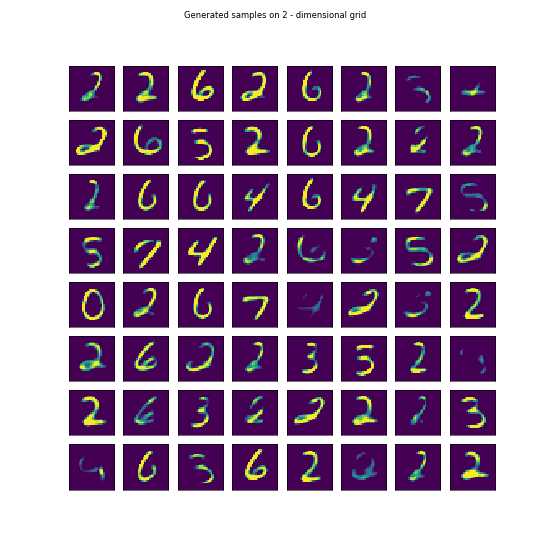
\includegraphics[width=.65\linewidth]{gen/generated_samples_mnist_dense_vae.png}
    \caption{Mintavételezett képek egy betanított $\beta$-VAE modellből, dense enkóder és dekóder architektúrával az MNIST adathalmazon}
    \label{fig:sampled-images-1}
  \end{minipage}\hfill
  \begin{minipage}{0.48\linewidth}
    \centering
    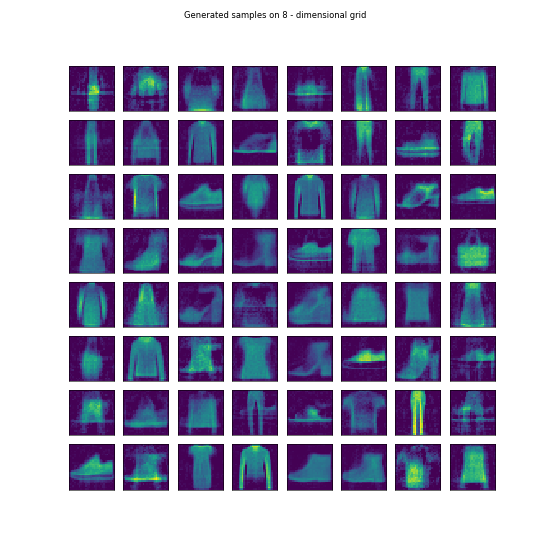
\includegraphics[width=.65\linewidth]{gen/generated_samples_fashion_mnist_dense_vae.png} 
    \caption{Mintavételezett képek egy betanított $\beta$-VAE modellből, dense enkóder és dekóder architektúrával a FashionMNIST} 
    \label{fig:sampled-images-2}
  \end{minipage} 
\end{figure}

\vspace{4mm}

\par Hogyan találhatunk rá egyáltalán a kontrasztot kódoló komponensre a látens kódban? Ahhoz, hogy ez lehetésgessé váljon korreláltuk a random kontraszt értékeket már a tanítás után a látensekkel és megnéztük, hogy még komponens korrelál a legjobban. Abszolútértékben 0.4 feletti korrelációnál már számítottunk arra, hogy sikerül függetleníteni a kontrasztot, mint látens komponens. Az LVAE architektúrában két látens kód is van, vizsgáltuk mindkettő korrelációját a kontrasztal és egymással is, hogy megtudjuk, hogy ugyanarra a stimulusra reagálnak-e a neuronok. Természetesen elsősorban lineáris korrelációkat vizsgáltunk, így ha magasabbrendű, nem lineáris összefüggés van a komponensek között, azt nem tudtuk ezzel dekódolni.

\vspace{4mm}

\subsection{Címke korrelációk vizsgálata}

\vspace{4mm}

\par Mivel ez egy nem felügyelt technika, de néhány adathalmaz tartalmazott címkéket így azok korrelációját is tudtuk vizsgálni a legmélyebb látens reprezentációkkal. Ilyen adathalmazok voltak például az MNIST, FashionMNIST az általunk főként vizsgált textúrák. Ezzel a módszerrel evidenssé vált, hogy melyik vált, hogy néhány címkére érzékenyebbek a modellek, mint másokra.

\vspace{4mm}

\begin{figure}[H]
    \centering
    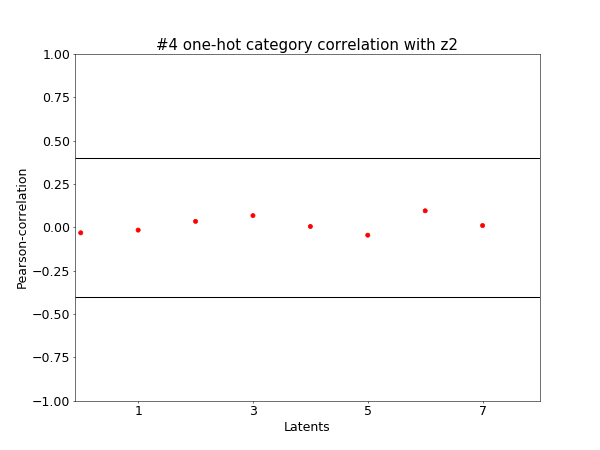
\includegraphics[width=0.55\textwidth]{17_DenseLinLinLadderVAE_contrastNorm-cat-4-to-z2-corr.png}
    \caption{Lineáris és dense enkóderek, dense és lineáris dekóderek - LVAE moell kontraszt normalizációval - a $4.$ komponens páronkénti korralációja $\bm{z^{(2)}}$-vel}
\end{figure}

\vspace{4mm}

\par Az LVAE architektúrában két sztochasztikus réteg van, ahol mintavételezni kell. A legmélyebb réteg a priorból mintavételezett, míg a köztes már tanult paraméterek alapján. Rendkíbül fontos vizsgálni, hogy ténylegesen megtörténik-e a hierarchikus reprezentáció, mert kellő komplexitású modellek segítségével a legmélyebb réteg elhagyható lehet, és csak zajt eredményez a rekonstrukciókon és nem kap értelmet a látens tér. Mivel a cél nem a rekonstrukciós pontosság, hanem ténylegesen az értelmes kódolás, erre külön figyelmet fordítottunk. Az implementációban hisztogrammokon lehet vizsgálni az átlagok és szórások eloszlását, amelyek a látens változók mintavételezéséhez szükségesek, továbbá divergáló színekkel a tényleges vektorok vizuális reprezentációját is megvalósítottuk, hogy lokalizáltan is követni lehessen, hogy hasonlóak-e a bennük tárolt értékek.

\vspace{4mm}

\begin{figure}[H]
    \centering
    
\includegraphics[width=0.3\textwidth]{diverging_color.png}
    \label{fig:diverging_colors}
    \caption{Divergens színek a vektor vizualizációkhoz}
\end{figure}

\vspace{4mm}

\subsection{UMAP beágyazás}

\vspace{4mm}

\par Vizsgáltuk még az UMAP \cite{mcinnes2018umap} és t-SNE \cite{maaten2008visualizing} beágyazásokat a látens reprezentációkon, hogy felmérjük, hogy vajon elválnak-e a textúra családok a látens térben. Fontos volt továbbá vizsgálnunk, hogy a hierarchikus reprezentáció különböző szintjein különböző, vagy ugyan az az információ van-e. Ezt a kérdést motiválja a \cite{ZiembaV2} cikk, ahol azt állítják, hogy a V2 más információt kódol, mint a V1. A számolási gyorsasága miatt az UMAP módszert alkalmaztam főkent, ami a t-SNE-hez hasonló beágyazásokat produkál, lényegesen gyorsabban. Különböző modelleket vizsgálva az LVAE architektúrában arra jutottunk, hogy látható, hogy különböző csoportok válnak el a két reprezentációban és más információ tárolódik:

\begin{figure}[H] 
  \begin{minipage}{0.48\linewidth}
    \centering
    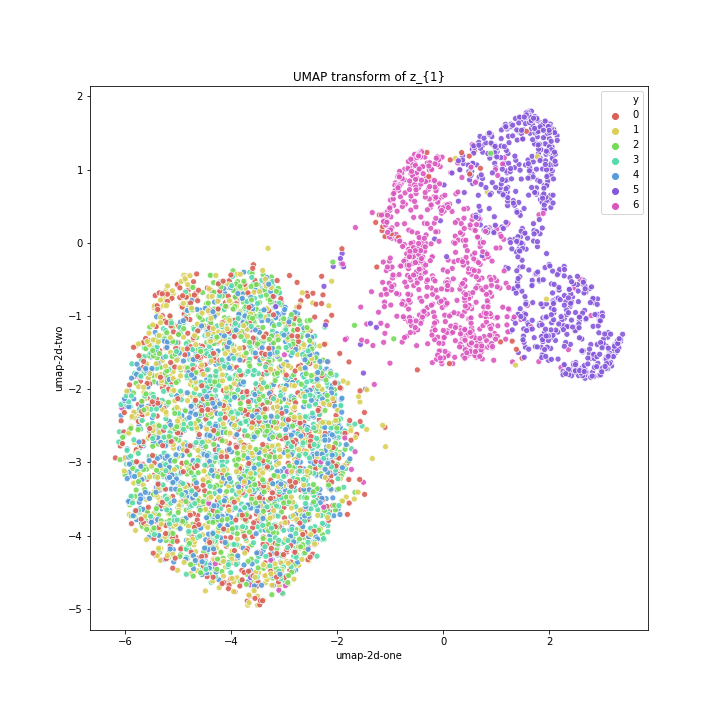
\includegraphics[width=.7\linewidth]{umap_z1_dense_lin_lin_no_norm.png}
    \caption{UMAP beagyazás $\bm{z^{(1)}}$-ből egy betanított LVAE architektúra lineáris és dense enkóderekkel, valamint dense és lineáris dekóderekkel}
    \label{fig:umap-z1}
  \end{minipage}\hfill
  \begin{minipage}{0.48\linewidth}
    \centering
    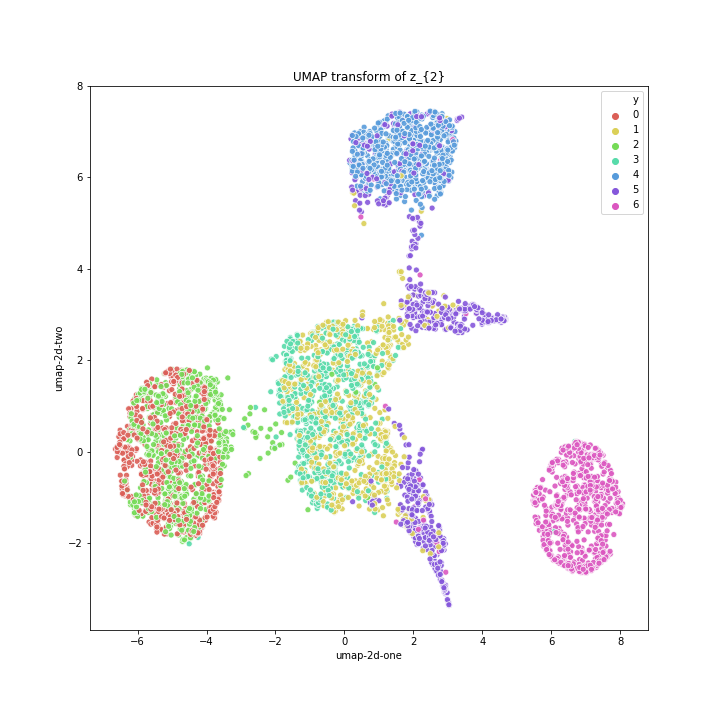
\includegraphics[width=.7\linewidth]{umap_z2_dense_lin_lin_no_norm.png} 
    \caption{UMAP beagyazás $\bm{z^{(2)}}$-ből egy betanított LVAE architektúra lineáris és dense enkóderekkel, valamint dense és lineáris dekóderekkel} 
    \label{fig:umap-z2}
  \end{minipage} 
\end{figure}

\vspace{4mm}

\par A dekompozíciók mellé, ahol a címkék láthatók elhelyezem a vizulálisan elkülöníthető képeket is a különböző textúrákről az UMAP beágyazásban. Az a tanulság szűrhető le ebből, hogy valamennyi információt a második enkóder almodell után sikerült elérni $\bm{z}^{(2)}$-ben, hiszen (\ref{fig:umap-z1}, \ref{fig:umap-z1-text}) láthatjuk az $5$, $6$ kategóriákat amelyek ténylegeen elkülönülnek két csoportba, míg az $5$ csoport három részre oszlott (\ref{fig:umap-z2}, \ref{fig:umap-z2-text})-n és már $3$-assal is elegyedett. Ezzel szemben, a legmélyebb rétegben már három csoport szeparálódik.

\vspace{4mm}

\begin{figure}[H] 
  \begin{minipage}{0.48\linewidth}
    \centering
    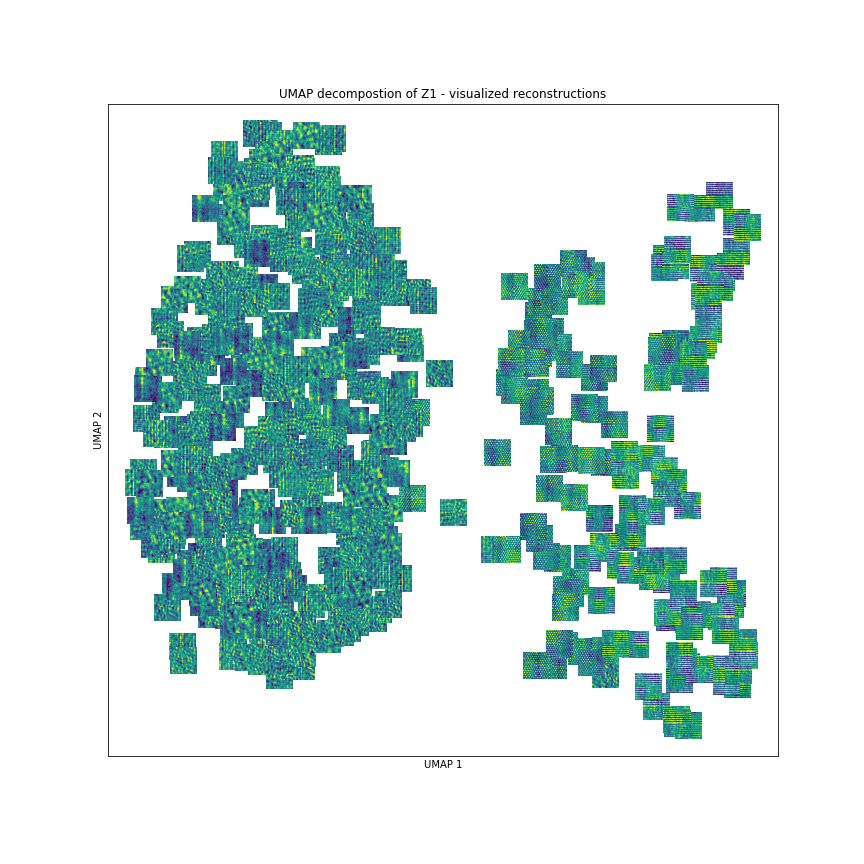
\includegraphics[width=.7\linewidth]{umap_z1_dense_lin_lin_no_norm_textures.png}
    \caption{UMAP beagyazás $\bm{z^{(1)}}$-ből egy betanított LVAE architektúra lineáris és dense enkóderekkel, valamint dense és lineáris dekóderekkel - a címkék helyett képek}
    \label{fig:umap-z1-text}
  \end{minipage}\hfill
  \begin{minipage}{0.48\linewidth}
    \centering
    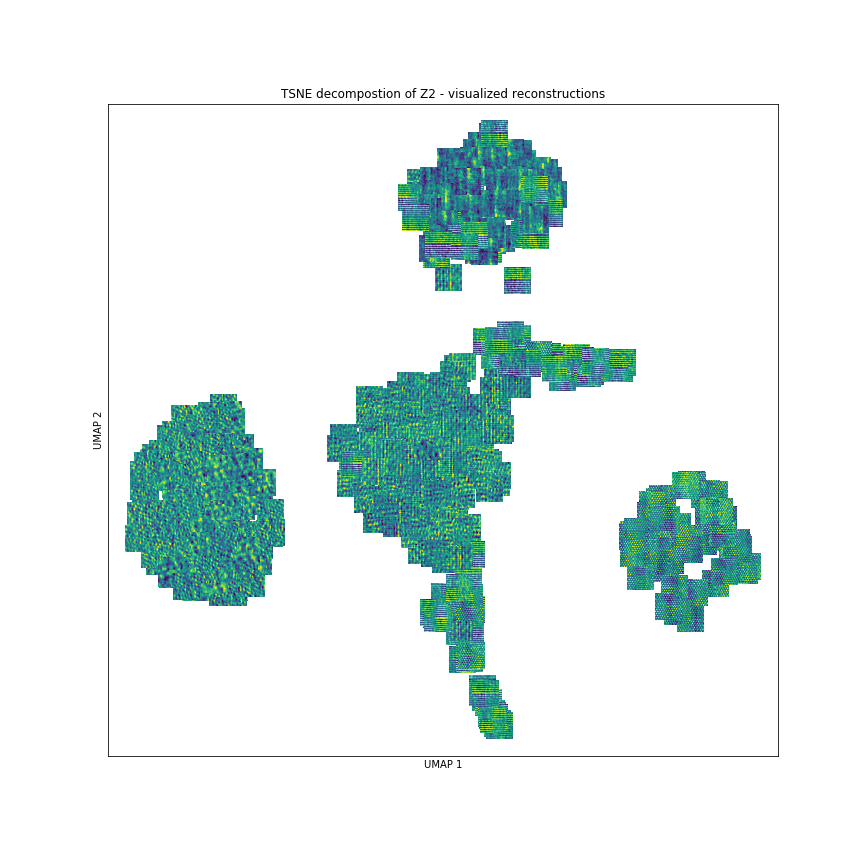
\includegraphics[width=.7\linewidth]{umap_z2_dense_lin_lin_no_norm_textures.png} 
    \caption{UMAP beagyazás $\bm{z^{(2)}}$-ből egy betanított LVAE architektúra lineáris és dense enkóderekkel, valamint dense és lineáris dekóderekkel - címkék helyett képek} 
    \label{fig:umap-z2-text}
  \end{minipage} 
\end{figure}

\vspace{4mm}

\par Páronkénti Pearson korrelációt is mértünk $\bm{z}^{(1)}$ és $\bm{z}^{(2)}$ között, amit úgy értünk el, hogy több ezer mintát korreláltattunk össze adott komponens aktivációra így kapva egy mátrixot, amiből azt találtuk, hogy lineáris korrelációk semmilyen esetben sincsenek a két látens kód között.

\vspace{4mm}

\begin{figure}[H]
    \centering
    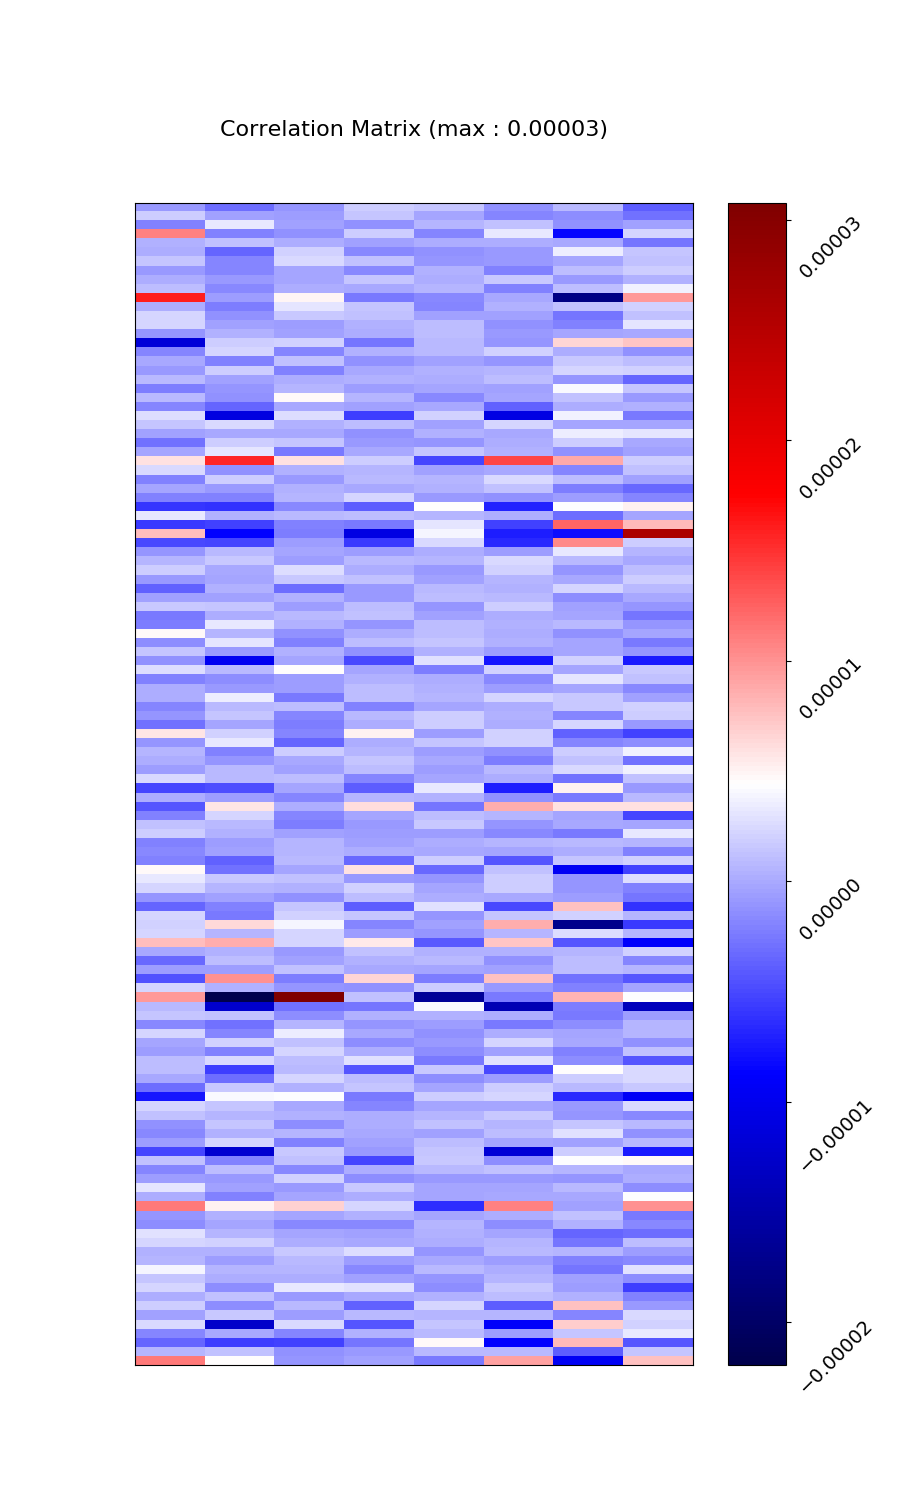
\includegraphics[width=0.3\textwidth]{z1_z2_correlation.png}
    \label{fig:pearson-matrix}
    \caption{Pearson-korreláció $\bm{z}^{(1)}$ és $\bm{z}^{(2)}$ között}
\end{figure}

\newpage

\section{Eredmények}

\vspace{7mm}

\subsection{Autoenkóderek}

\vspace{5mm}

\par Auto-encoders are not generative models but non-linear functions that are learning to reconstruct unlabelled data by pushing it through a usually reduced dimensionality gate. This low-dimensional representation with the decoder architecture can be ported to everywhere and for large datasets it can save much more space than regular compression tools such as JPEG. It is important to mention that compression via auto-encoders is highly dataset specific so it cannot be used as conveniently as JPEG without training a neural network. Also, the compression is lossy so the images cannot be fully reconstructed without some information loss.

\vspace{4mm}

\par Results are presented using the well-known MNIST dataset with binarized values and Bernoulli-loss:

\vspace{4mm}

\begin{figure}[H] 
  \label{fig:auto_encoder_results} 
  \begin{minipage}{0.48\linewidth}
    \centering
    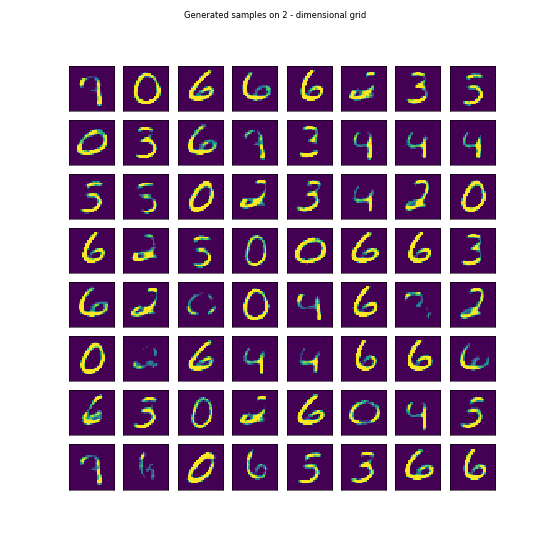
\includegraphics[width=.65\linewidth]{gen/generated_samples_mnist_auto_encoder.png} 
    \caption{Sampled images} 
  \end{minipage}\hfill
  \begin{minipage}{0.48\linewidth}
    \centering
    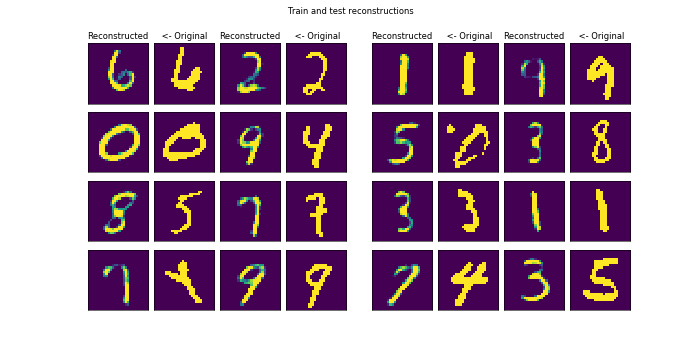
\includegraphics[width=.95\linewidth]{reco/reconstrunction_samples_mnist_auto_encoder.png} 
    \caption{Reconstructed images} 
  \end{minipage} 
\end{figure}

\vspace{4mm}

\par The latent representation contained length two vectors and it can be seen that such low complexity data is well represented even without constraint on the code.

\newpage

\subsection{Variációs autoenkóderek}

\vspace{5mm}

\par Results are presented using the Fashion-MNIST dataset with continuous pixel values in $[0, 1]$ and normal loss the model used is presented in (\ref{fig:dense-variational-auto-encoder} - see appendix \ref{sec:vae}):

\vspace{4mm}

\begin{figure}[ht] 
  \label{fig:auto_encoder_results} 
  \begin{minipage}{0.5\linewidth}
    \centering
    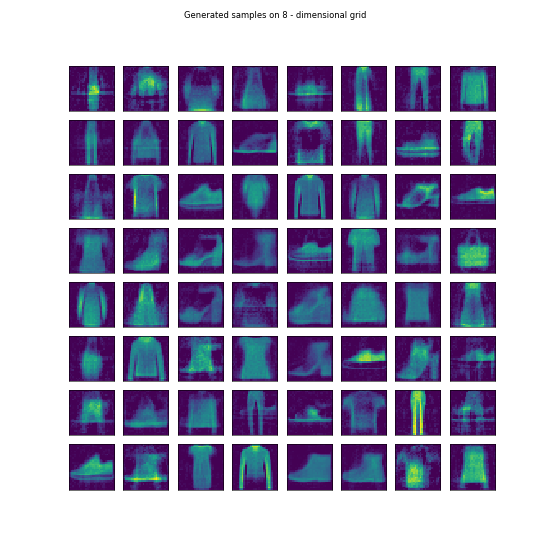
\includegraphics[width=.65\linewidth]{gen/generated_samples_fashion_mnist_dense_vae.png} 
    \caption{Sampled images} 
  \end{minipage}%%
  \begin{minipage}{0.5\linewidth}
    \centering
    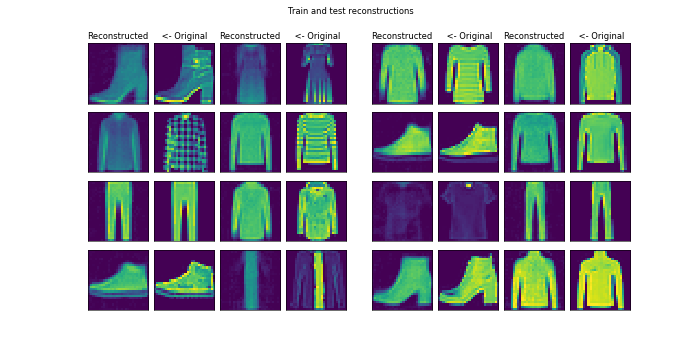
\includegraphics[width=.95\linewidth]{reco/reconstrunction_samples_fashion_mnist_dense_vae.png} 
    \caption{Reconstructed images} 
  \end{minipage} 
\end{figure}

\vspace{4mm}

\par The latent representation contained length eight vectors and it was trained with $\beta = 1$.

\vspace{4mm}

\par Using the same eight piece code and the same training iterations, the effect of the variational inference can be seen in the latent representation compared to the non-variational model (\ref{fig:dense-auto-encoder} - see appendix \ref{sec:auto-encoder}):

\begin{figure}[ht] 
  \label{fig:auto_encoder_results} 
  \begin{minipage}{0.5\linewidth}
    \centering
    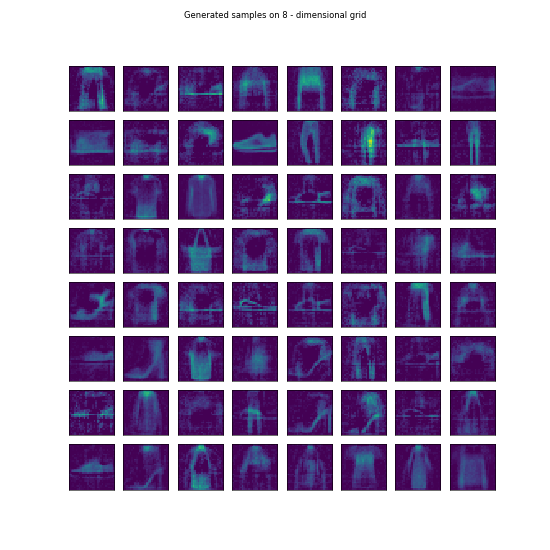
\includegraphics[width=.65\linewidth]{gen/generated_samples_fashion_mnist_auto_encoder.png} 
    \caption{Sampled images} 
  \end{minipage}%%
  \begin{minipage}{0.5\linewidth}
    \centering
    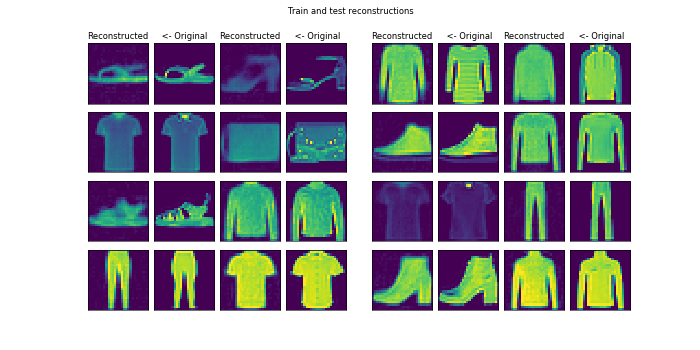
\includegraphics[width=.95\linewidth]{reco/reconstrunction_samples_fashion_mnist_auto_encoder.png} 
    \caption{Reconstructed images} 
  \end{minipage} 
\end{figure}

\vspace{4mm}

\par In the reconstructions the effect cannot be seen but it is easily observed in the latent representation since it is less pronounced in the non-variational model.

\newpage

\subsection{Létra variációs autoenkóderek}

\vspace{5mm}

\par The ladder architecture introduces an additional layer of abstraction into our variational model. Better latent representations are expected using this as our model.

\vspace{4mm}

\par Training a deeper model poses difficulties since training it efficiently is much harder and usually many more iterations are needed. Since randomly initialized weights might provide a very bad spot on the loss landscape the deviation in the KL-term can be very high and latent representations are basically non-existent. The connection between the bottom up and top down components at the intermediate layer also poses a threat since information sharing provides a loophole to the model not to abstract information and just leave the deeper stochastic code out of the process. 

\vspace{4mm}

\par This effect can be handled in a few different ways such as: restricting the encoders first layer to be linear and the decoder at the top to be linear as well, this results in forcing the models to use deeper layers since a very low level of abstraction can be achieved with such low complexity models. A higher $\beta_{max}$ can achieve similar effect since the KL-term can influence the overall loss more and could also force the model to use deeper representations in order to lower the KL-loss significantly. 

\vspace{4mm}

\par In the following sections I mostly used different architectures of LVAEs with constrained linear encoders and decoders and with dense encoders and decoders.

\vspace{7mm}

\subsection{A függetlenített kontraszt reprezentáció megértése}

\vspace{5mm}

\par As I mentioned previously, I implemented random contrast learning, meaning that some random amount of contrast is added to each batch of the input images to make the model contrast independent in order to disentangle the contrast in the latent code. I looked into what is necessary in order to acquire such disentangled representation in \cite{locatello2018challenging} researchers at Google did most of this work from a computer science perspective and they concluded that only inductive biases, such as architectural choice, different regularization and loss terms make disentangled representations possible. Here I attempt to understand what is needed to disentangle contrast from these textural images.

\vspace{4mm}

\subsubsection{LVAE I.}

\vspace{4mm}

\par Here I present some results with linear modules at the first encoder and last decoder layer (\ref{fig:linlinladdervae} - see appendix \ref{sec:lvae1}) with and without contrast normalization with the same settings: $[\bm{z}_{1}] = 128, [\bm{z}_{2}] = 8$:

\vspace{4mm}

\begin{figure}[H] 
  \begin{minipage}{0.5\linewidth}
    \centering
    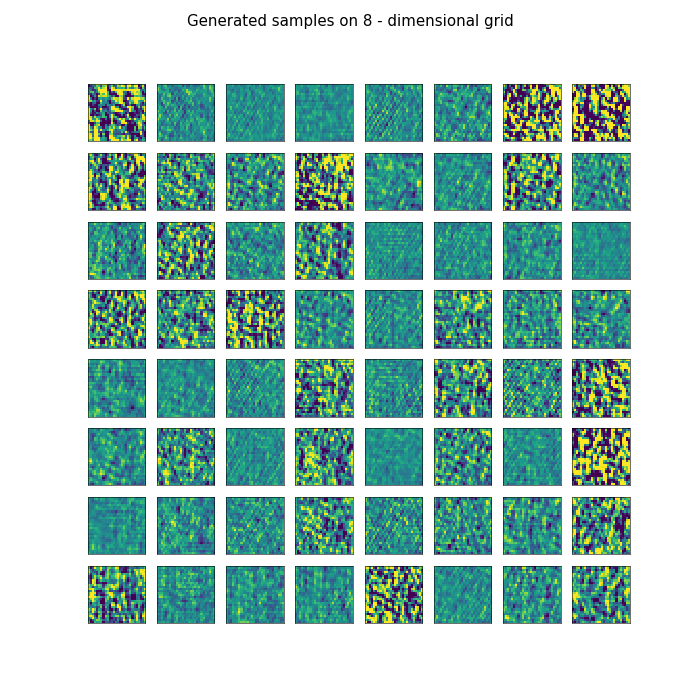
\includegraphics[width=.75\linewidth]{contrast/generated_samples_noContrastNorm_noContrast.png} 
    \caption{No contrast - no normalization} 
    \label{fig:contrast-generated-1} 
  \end{minipage}%%
  \begin{minipage}{0.5\linewidth}
    \centering
    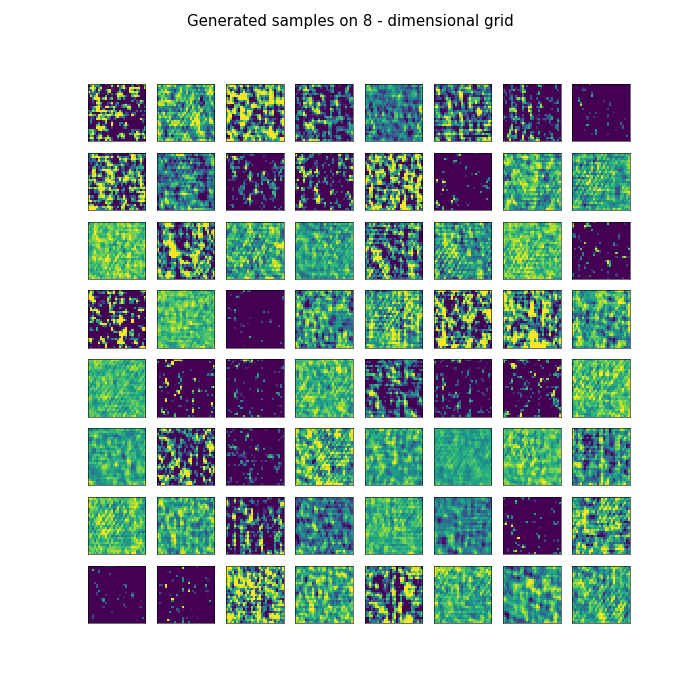
\includegraphics[width=.75\linewidth]{contrast/generated_samples_noContrastNorm_contrast.png} 
    \caption{Contrast - no normalization} 
    \label{fig:contrast-generated-2} 
  \end{minipage} 
  \begin{minipage}{0.5\linewidth}
    \centering
    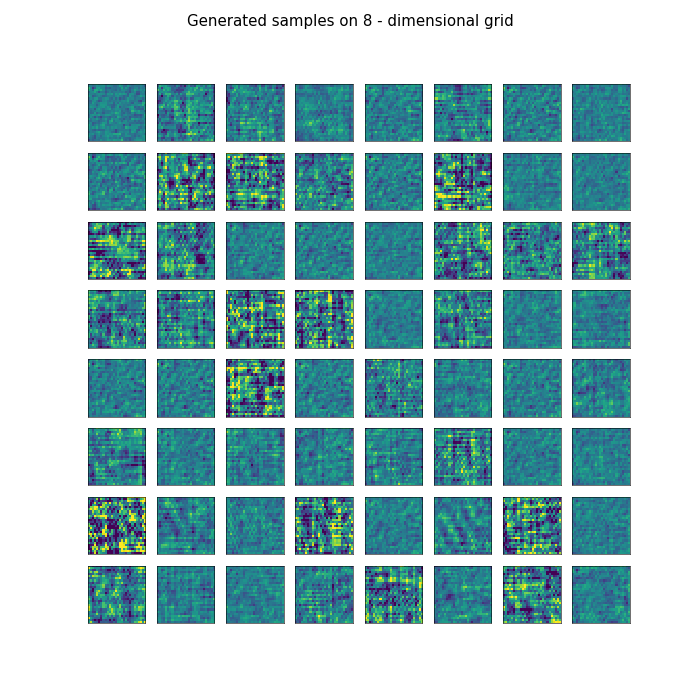
\includegraphics[width=.75\linewidth]{contrast/generated_samples_contrastNorm_noContrast.png} 
    \caption{No contrast - normalization} 
    \label{fig:contrast-generated-3} 
  \end{minipage}%% 
  \begin{minipage}{0.5\linewidth}
    \centering
    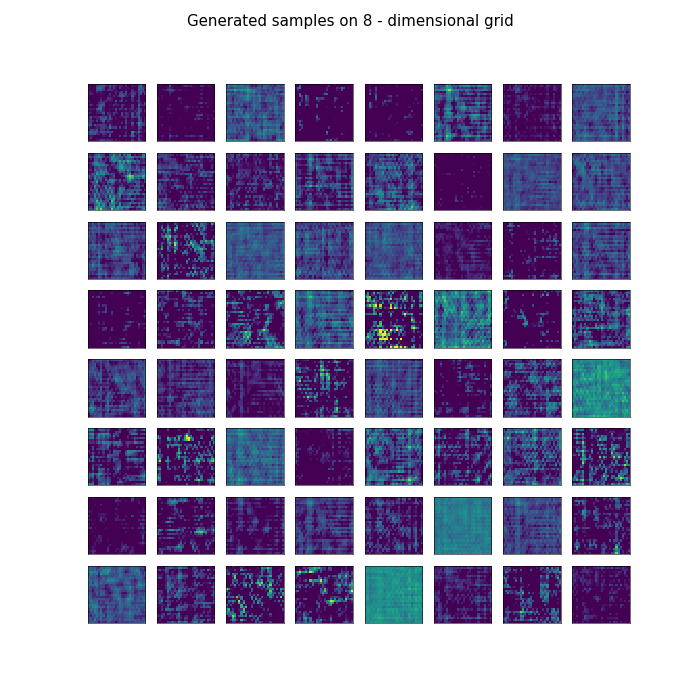
\includegraphics[width=.75\linewidth]{contrast/generated_samples_contrastNorm_contrast.png} 
    \caption{Contrast - normalization} 
    \label{fig:contrast-generated-4} 
  \end{minipage} 
\end{figure}

\vspace{4mm}

\par What we can see in (\ref{fig:contrast-generated-1}, \ref{fig:contrast-generated-2}, \ref{fig:contrast-generated-3},\ref{fig:contrast-generated-4}) is not trivial to compare, however, just by looking at them we can see how contrast modifies training, since we can observe large variance in contrast amongst the generated textures and also normalization can be observed in contrast of images.

\vspace{4mm}

\par A more thorough and systematic comparison can be gained by comparing contrast correlation with the latent codes. This can be done by generating random contrast values. Assuming a batch size $B_{s}$ and latent code dimension $d$ we can correlate the latent code at index $i$ of each element in the batch $z^{(i)}_{\{j\}_{j = 1}^{B_{s}}}$ with the random contrast values of the batch. Calculating simple Pearson-correlation:

\vspace{4mm}

\begin{equation*}
    \rho(\bm{z}^{(i)}, \bm{R_{c}}) = \frac{Cov(\bm{z}^{(i)}, \bm{R_{c}})}{\sigma(\bm{z}^{(i)})\sigma(\bm{R_{c}})}  
\end{equation*}

\vspace{4mm}

\par In this form both the random contrast $\bm{R_{c}}$ and the $i$th component of the latent code for each element in the batch $\bm{z}^{(i)}$ have size $B_{s}$, so comparing these for each of the contrast-normalization models:

\vspace{4mm}

\begin{figure}[H] 
  \label{fig:contrast-correlation} 
  \begin{minipage}{0.5\linewidth}
    \centering
    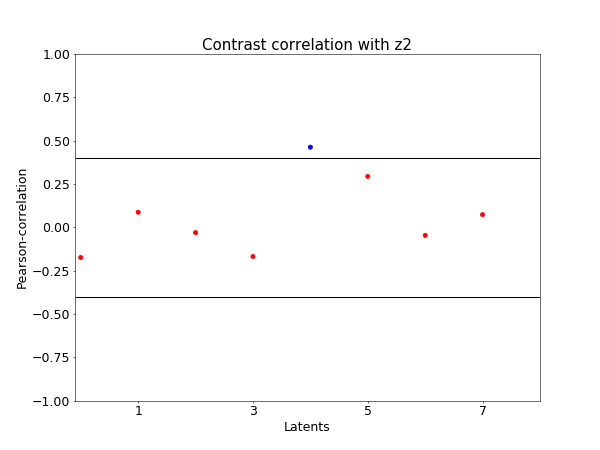
\includegraphics[width=.72\linewidth]{contrast_to_latent/no_norm_contrast_z2_corr.png} 
    \caption{No contrast - no normalization} 
    \label{fig:no-contrast-no-norm}
  \end{minipage}%%
  \begin{minipage}{0.5\linewidth}
    \centering
    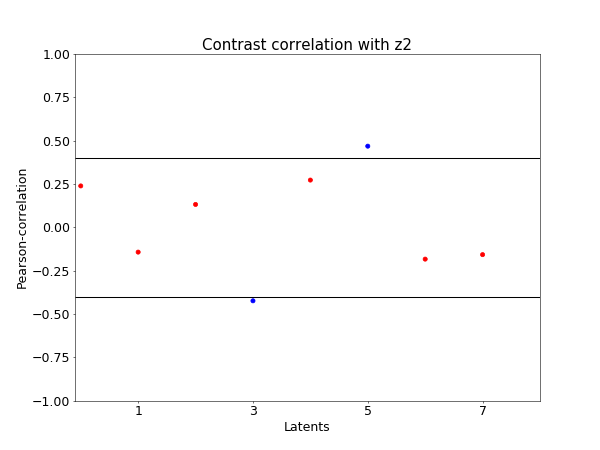
\includegraphics[width=.72\linewidth]{contrast_to_latent/no_norm_contrast_contrast_z2_corr.png} 
    \caption{Contrast - no normalization} 
    \label{fig:contrast-no-norm}
  \end{minipage} 
  \begin{minipage}{0.5\linewidth}
    \centering
    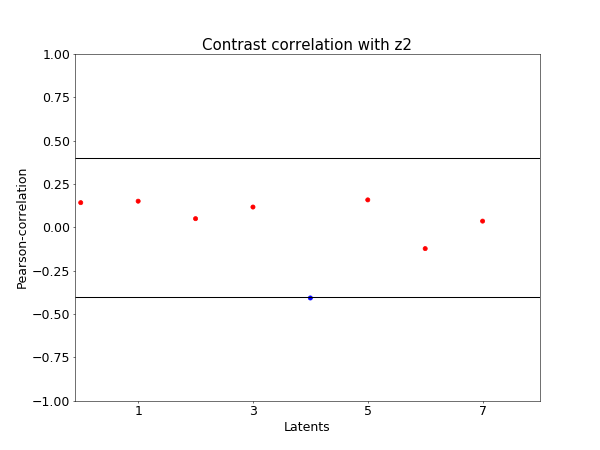
\includegraphics[width=.72\linewidth]{contrast_to_latent/norm_no_contrast_correlation.png} 
    \caption{No contrast - normalization} 
    \label{fig:no-contrast-norm}
  \end{minipage}%% 
  \begin{minipage}{0.5\linewidth}
    \centering
    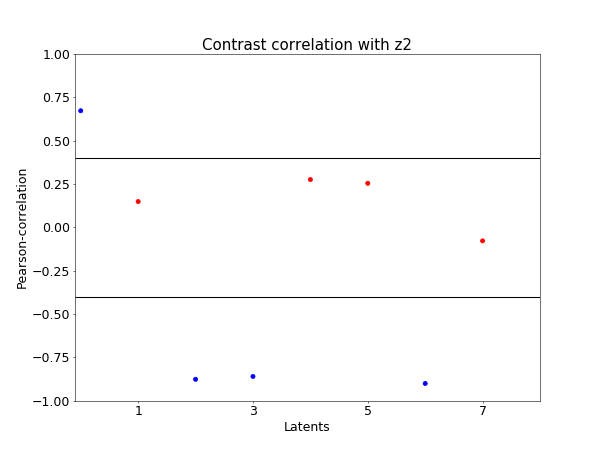
\includegraphics[width=.72\linewidth]{contrast_to_latent/norm_contrast_correlation.png} 
    \caption{Contrast - normalization} 
    \label{fig:contrast-norm}
  \end{minipage} 
\end{figure}

\vspace{4mm}

\par Here we can see that in (\ref{fig:no-contrast-no-norm}) there seems to be natural contrast in this type of dataset and it seems to be disentangled in the $4$th latent code component \footnote{indexing from $0$}. I'll also analyze whether this is the case or the latent code represents a class that has high variability in contrast and only disentangles that class. Adding additional contrast (\ref{fig:contrast-no-norm}) to the textures made two variables to encode something like contrast.

\vspace{4mm}

\par The case is very similar with contrast normalization (\ref{fig:no-contrast-norm}, \ref{fig:contrast-norm}) although this is not expected. This could mean that contrast normalization failed or that the parameter that is seemingly encodes contrast \footnote{has high correlation with what we call contrast} actually encodes a class that has high variability locally even though it was globally normalized.

\vspace{4mm}

\par Observing the labels and their correlation with the deepest latent code $\bm{z}_{2}$ I found that the correlation in each variable with respect to the contrast or the one-hot-encoded $1$st label is almost the same in the non normalized setting:

\vspace{4mm}

\begin{figure}[H]
\begin{minipage}{0.5\linewidth}
    \centering
    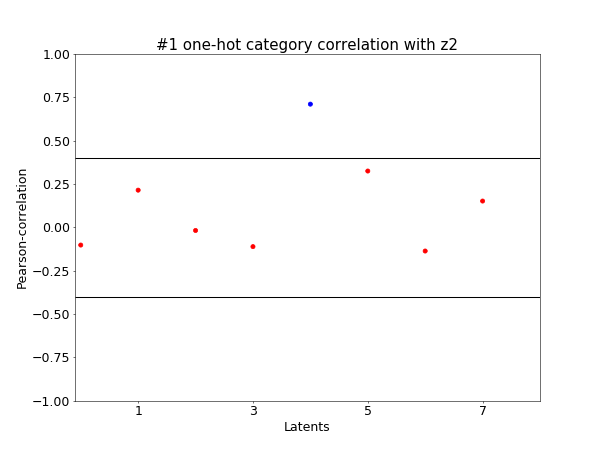
\includegraphics[width=.72\linewidth]{label-contrast-corr/cat-1-to-z2-corr.png} 
    \caption{$1$st one-hot encoded label to $\bm{z}_{2}$} 
    \label{fig:label-contrast-corr-1}
\end{minipage}%% 
\begin{minipage}{0.5\linewidth}
    \centering
    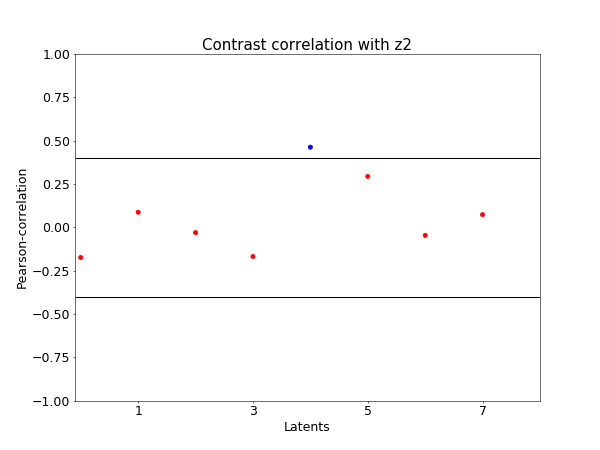
\includegraphics[width=.72\linewidth]{label-contrast-corr/contrast-to-z2-corr.png} 
    \caption{Contrast to $\bm{z}_{2}$} 
    \label{fig:label-contrast-corr-2}
\end{minipage} 
\end{figure}

\par With the non-normalized setting when there is additional contrast there are also high correlations with some of the one-hot-encoded labels therefore no clean disentanglement is provided by the latent representation.

\vspace{4mm}

\par However, another observation can be made by checking that normalized setting. In this scenario the label correlations with $\bm{z}_{2}$ are negligible in both cases of no contrast and additional contrast during training. This leads me to believe that the parameter that correlates with the additional contrast during reconstruction is encoding the local contrast in the normalized scenario. To test this I mentioned earlier that I implemented latent sweep in my code base. Also I made sure that I the latent codes are used in the trained models by observing there means and standard deviations during reconstruction, if these are different from zero and one respectively, meaning that they are not unit Gaussians but some kind of learnt posteriors the models are actually using them for something.

\vspace{4mm}

\begin{figure}[H] 
  \label{fig:contrast-correlation} 
  \begin{minipage}{0.33\linewidth}
    \centering
    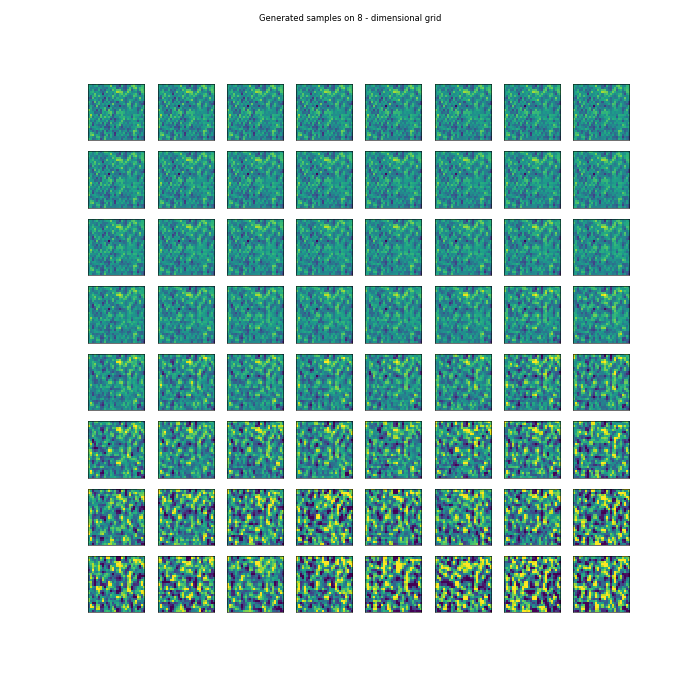
\includegraphics[width=.72\linewidth]{sweep/no_norm_no_contrast_sweep_minus_two_to_one.png} 
    \caption{No contrast, no \newline norm. sweep in $[-2, 1]$} 
    \label{fig:no-contrast-no-norm-sweep}
  \end{minipage}%%
  \begin{minipage}{0.33\linewidth}
    \centering
    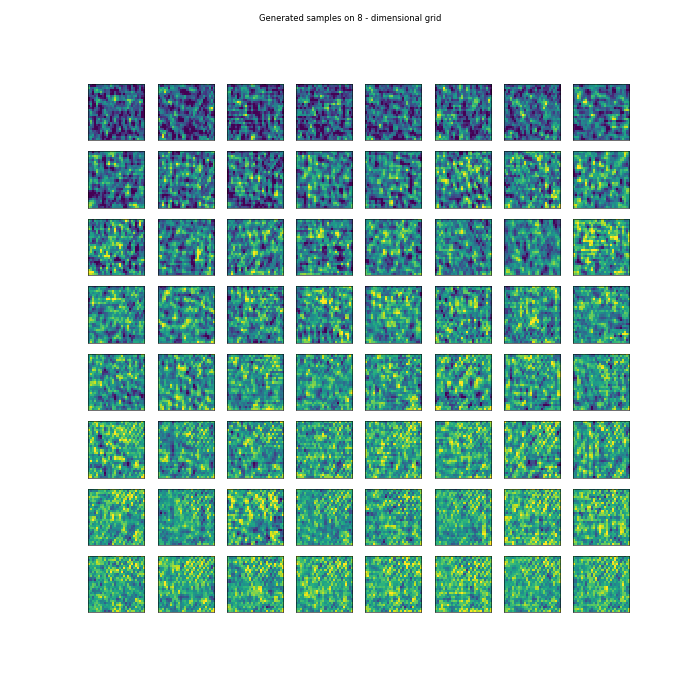
\includegraphics[width=.72\linewidth]{sweep/no_norm_contrast_sweep_minus_two_to_two_3rd_param.png} 
    \caption{Contrast, no norm. \newline sweep in $[-2, 2]$ $3$rd component} 
    \label{fig:contrast-no-norm-sweep-3}
  \end{minipage} 
  \begin{minipage}{0.33\linewidth}
    \centering
    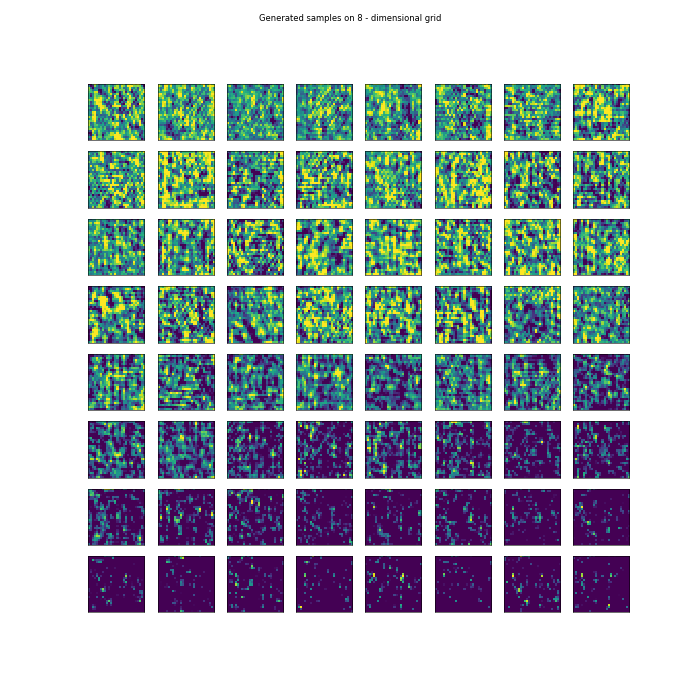
\includegraphics[width=.72\linewidth]{sweep/no_norm_contrast_sweep_minus_two_to_two_5th_param.png} 
    \caption{Contrast, no norm. \newline sweep in $[-2, 2]$ $5$th component} 
    \label{fig:contrast-no-norm-sweep-5}
  \end{minipage}
  %% stats
  \begin{minipage}{0.5\linewidth}
    \centering
    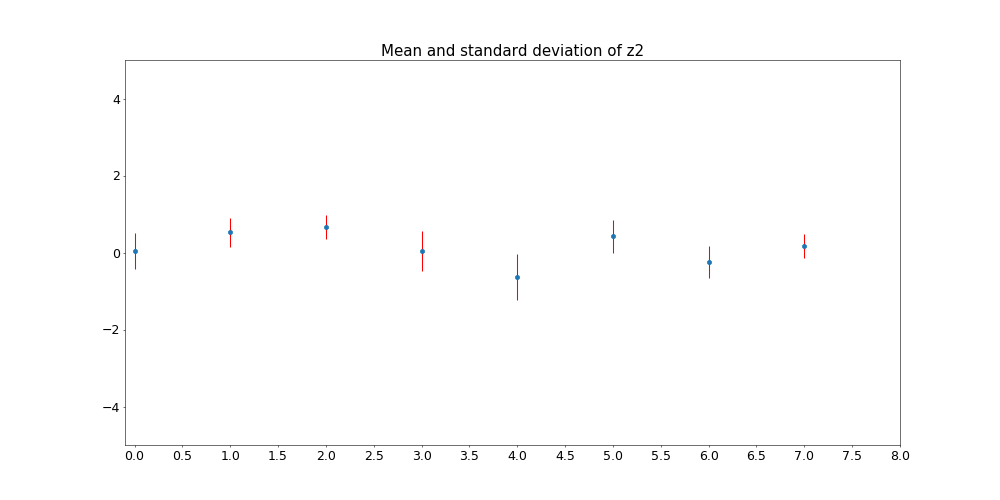
\includegraphics[width=.95\linewidth]{sweep/no_contrast_no_norm_z2_stats.png} 
    \caption{No contrast \newline no norm $\bm{z}_{2}$ statistics} 
    \label{fig:no-contrast-no-norm-stats}
  \end{minipage} 
  \begin{minipage}{0.5\linewidth}
    \centering
    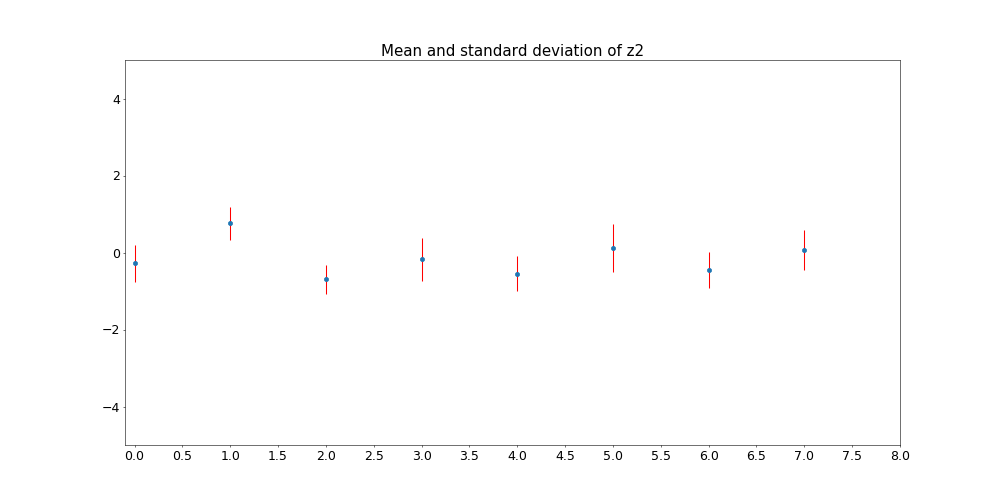
\includegraphics[width=.95\linewidth]{sweep/contrast_no_norm_z2_stats.png} 
    \caption{Contrast, no norm. \newline $\bm{z}_{2}$ statistics} 
    \label{fig:contrast-no-norm-stats}
  \end{minipage}
\end{figure}

\vspace{4mm}

\par With the non-normalized settings in (\ref{fig:no-contrast-no-norm-sweep}) the latent component $4$ is selected from (\ref{fig:no-contrast-no-norm}) with regard to its mean and deviation from (\ref{fig:no-contrast-no-norm-stats}), sweeping therefore in the almost $2\sigma$ range $[-2, 1]$ in the fourth component results in generated samples differing not mostly in contrast but at the bottom \footnote{since generation was done in row flattened order, this means that closer to the right end of the spectrum} of (\ref{fig:no-contrast-no-norm-sweep}) results in a class resembling the $1$st label what we expected (\ref{fig:label-contrast-corr-1}, \ref{fig:label-contrast-corr-2}). However, when contrast is introduced (\ref{fig:contrast-no-norm-sweep-3}, \ref{fig:contrast-no-norm-sweep-5}) still there are high correlations with the one-hot encoded labels, so we could not get a truly disentangled contrast representation in the latent components. On the other hand what we can see in these generated samples that the $3$rd and $5$th components that have high correlation with the random contrast (\ref{fig:contrast-no-norm}) resulted in high contrast images, especially in (\ref{fig:contrast-no-norm-sweep-5}).

\vspace{4mm}

\par Moving on to the normalized scenario:

\vspace{4mm}

\begin{figure}[H] 
  \label{fig:contrast-correlation} 
  \begin{minipage}{0.4\linewidth}
    \centering
    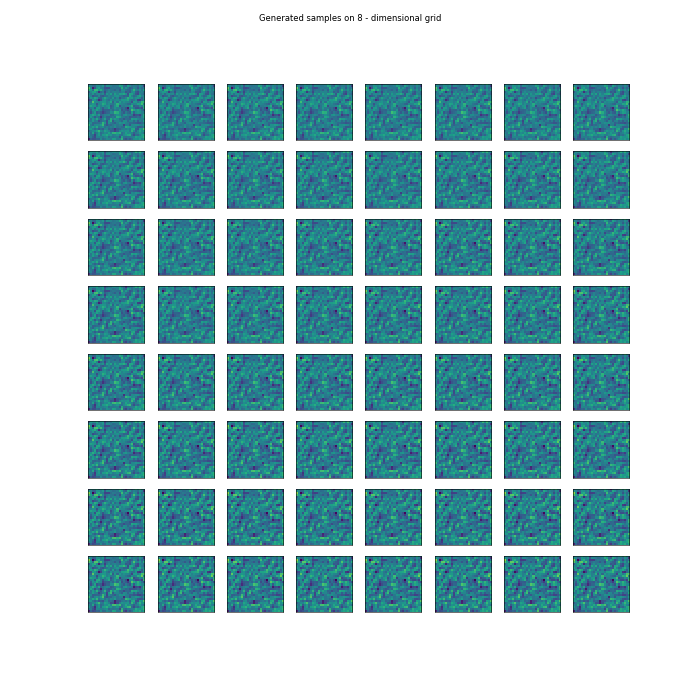
\includegraphics[width=.8\linewidth]{sweep/norm_no_contrast_sweep_one_to_two_4th_param.png} 
    \caption{No contrast, norm., sweep in $[1, 2]$, $4$th compoment} 
    \label{fig:no-contrast-norm-sweep}
  \end{minipage}%%
  \begin{minipage}{0.6\linewidth}
    \centering
    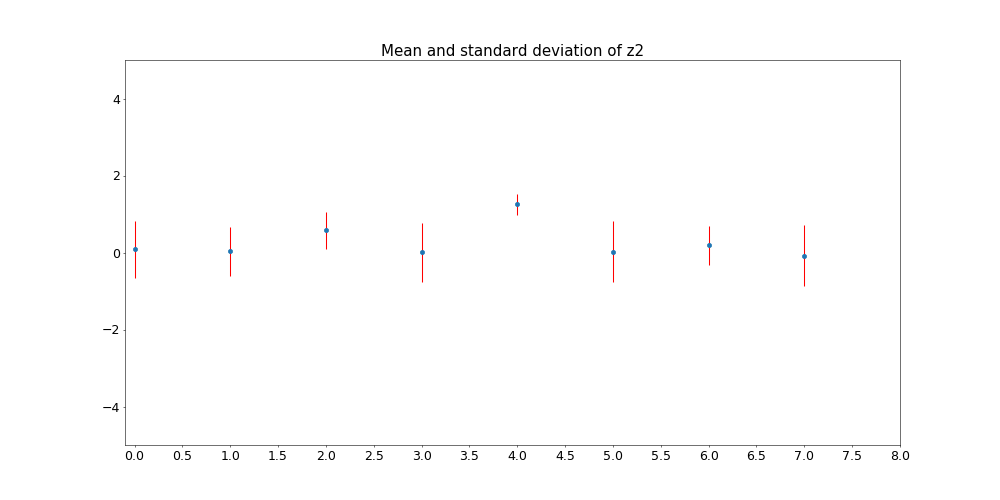
\includegraphics[width=1\linewidth]{sweep/norm_no_contrast_z2_stats.png} 
    \caption{No contrast, norm.,  $\bm{z}_{2}$ statistics} 
    \label{fig:no-contrast-no-norm-stats}
  \end{minipage} 
\end{figure}

\vspace{4mm} 
 
\par  These generated samples with sweeping suggests that the correlations of the $4$th component with the random contrast values in (\ref{fig:no-contrast-norm}) is not high enough, therefore it is not encoding contrast at all. In (\ref{fig:no-contrast-norm-sweep}) there are no trivial differences across the sweep so it is unknown what the component actually encodes. Adding additional contrast to normalized images results in:

\vspace{4mm}
 
\begin{figure}[H]
  \begin{minipage}{0.5\linewidth}
    \centering
    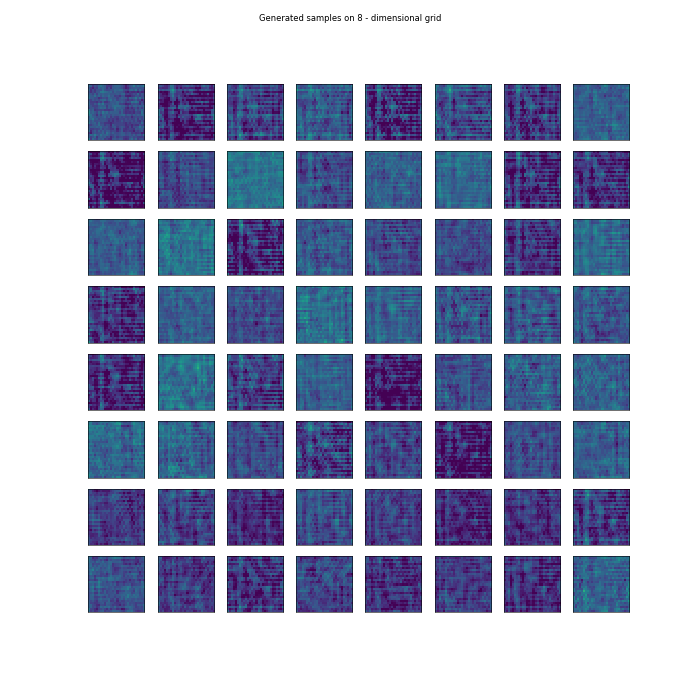
\includegraphics[width=.85\linewidth]{sweep/norm_contrast_sweep_zero_to_one_0th_param.png} 
    \caption{Contrast, norm., sweep in $[0, 1]$ \newline $0$th component} 
    \label{fig:contrast-norm-sweep-0}
  \end{minipage} 
  \begin{minipage}{0.5\linewidth}
    \centering
    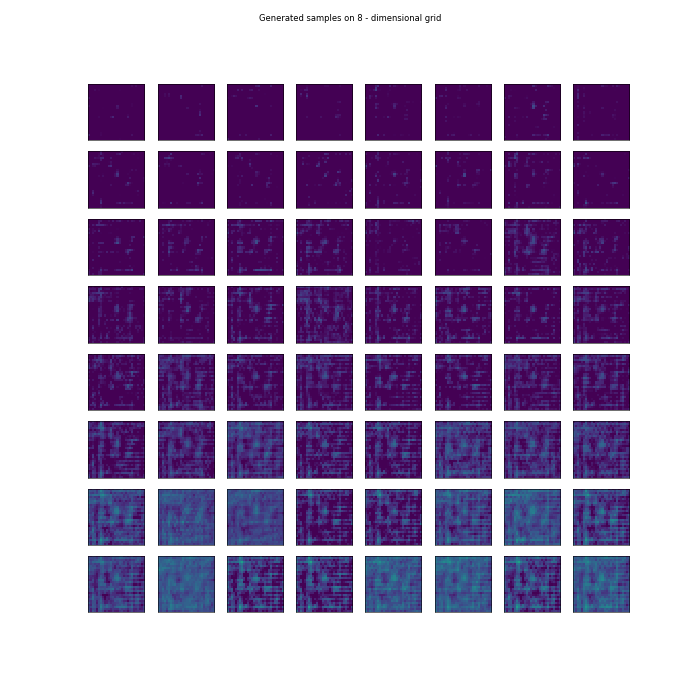
\includegraphics[width=.85\linewidth]{sweep/norm_contrast_sweep_minus_two_to_one_2nd_param.png} 
    \caption{Contrast, norm., sweep in $[-2, 1]$ \newline $2$nd component} 
    \label{fig:contrast-norm-sweep-2}
  \end{minipage}
\end{figure}


\begin{figure}[H]
  \begin{minipage}{0.5\linewidth}
    \centering
    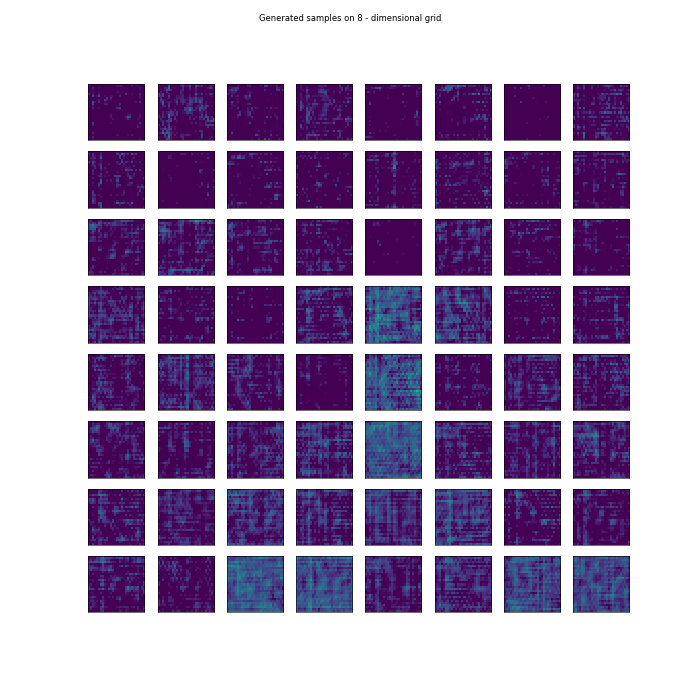
\includegraphics[width=.85\linewidth]{sweep/norm_contrast_sweep_minus_two_to_one_3rd_param.png} 
    \caption{Contrast, norm., sweep in $[-2, 1]$ \newline  $3$rd component} 
    \label{fig:contrast-norm-sweep-3}
  \end{minipage}
  \begin{minipage}{0.5\linewidth}
    \centering
    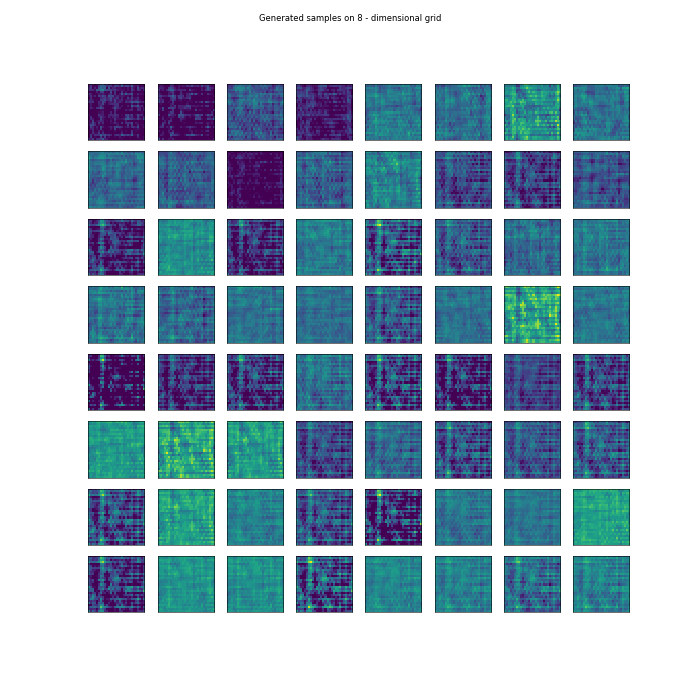
\includegraphics[width=.85\linewidth]{sweep/norm_contrast_sweep_zero_to_two_6th_param.png} 
    \caption{Contrast, norm., sweep in $[0, 2]$ \newline $6$th component} 
    \label{fig:contrast-norm-sweep-6}
  \end{minipage}
\end{figure}

\begin{figure}[H]
    \centering
    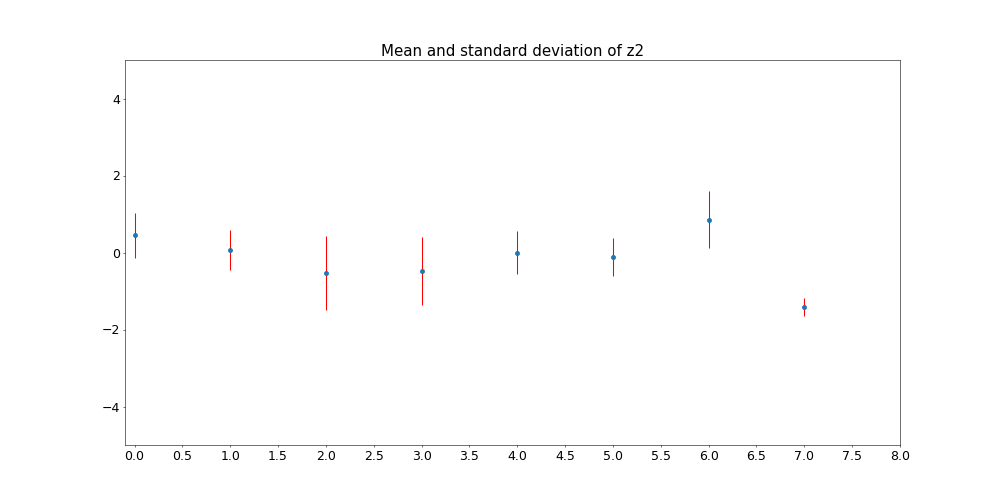
\includegraphics[width=.85\linewidth]{sweep/norm_contrast_z2_stats.png} 
    \caption{Contrast, norm., $\bm{z}_2$ statistics} 
    \label{fig:contrast-norm-stats}
\end{figure}

\vspace{4mm}

\par The components were selected from the corresponding contrast correlation plot (\ref{fig:contrast-norm}) and their ranges very selected from (\ref{fig:contrast-norm-stats}) to approximately cover $2\sigma$ range of the mean. We expect gradual contrast increment in row wise order but this can only be seen vaguely on (\ref{fig:contrast-norm-sweep-2}) but not in the others.

\vspace{4mm}

\subsubsection{LVAE II.}

\vspace{4mm}

\par In the previous section we used a ladder variational auto-encoder with constrained linear encoder and decoder, here we use the same settings for training with the same data manipulations and attempt to see the differences.

\vspace{4mm}

\begin{figure}[H] 
  \begin{minipage}{0.5\linewidth}
    \centering
    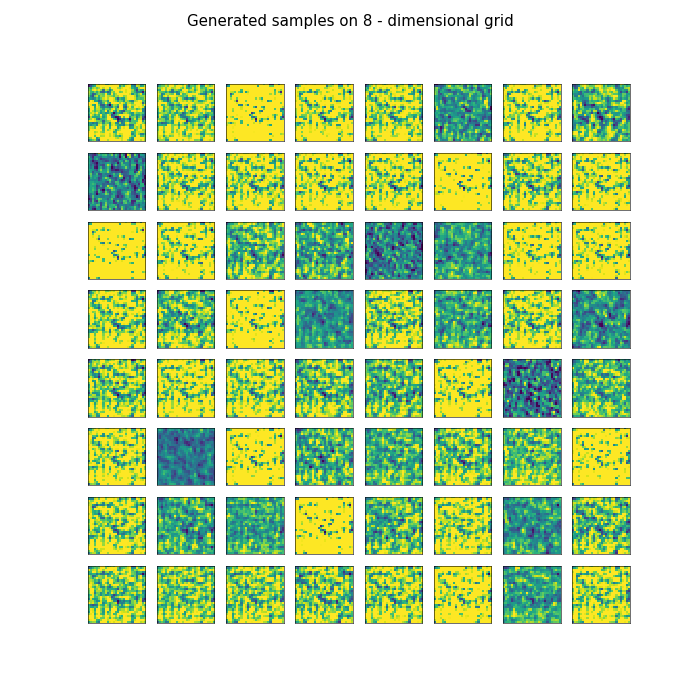
\includegraphics[width=.75\linewidth]{lvae2/21_DenseLadderVAE_noNorm-generated_samples.png} 
    \caption{No contrast - no normalization} 
    \label{fig:lvae-2-contrast-generated-1} 
  \end{minipage}%%
  \begin{minipage}{0.5\linewidth}
    \centering
    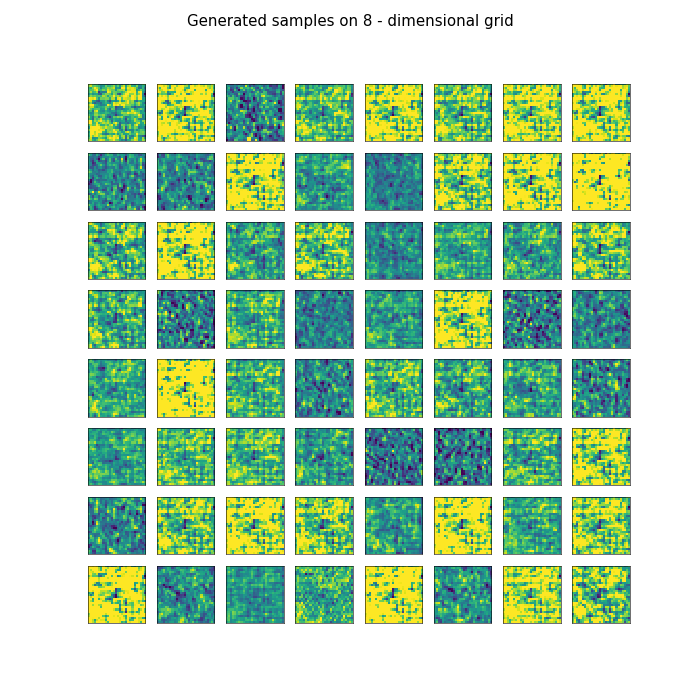
\includegraphics[width=.75\linewidth]{lvae2/20_DenseLadderVAE_noNorm_contrat-generated_samples.png} 
    \caption{Contrast - no normalization} 
    \label{fig:lvae-2-contrast-generated-2} 
  \end{minipage} 
  \begin{minipage}{0.5\linewidth}
    \centering
    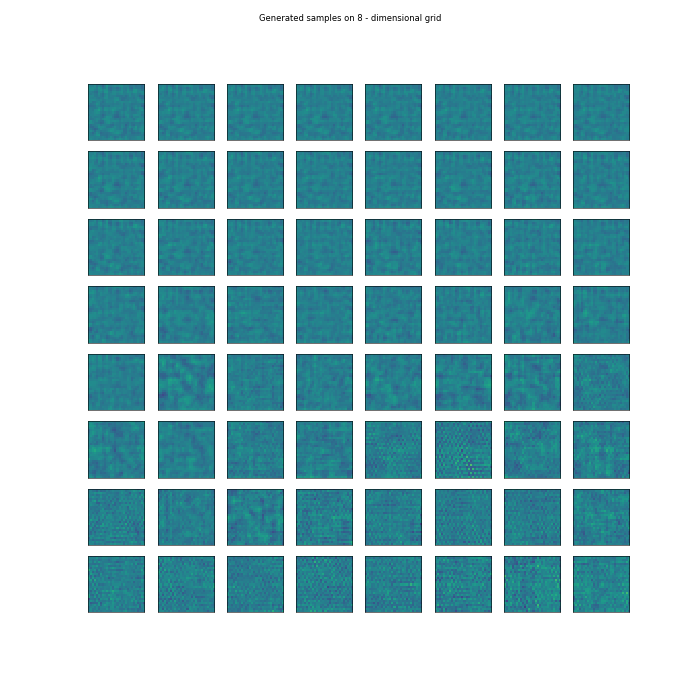
\includegraphics[width=.75\linewidth]{lvae2/18_DenseLadderVAE_contrastNorm-generated_samples.png} 
    \caption{No contrast - normalization} 
    \label{fig:lvae-2-contrast-generated-3} 
  \end{minipage}%% 
  \begin{minipage}{0.5\linewidth}
    \centering
    \includegraphics[width=.75\linewidth]{lvae2/19_DenseLadderVAE_contrastNorm_contrast-generated_samples.png} 
    \caption{Contrast - normalization} 
    \label{fig:lvae-2-contrast-generated-4} 
  \end{minipage} 
\end{figure}

\vspace{4mm}

\par In (\ref{fig:lvae-2-contrast-generated-1}, \ref{fig:lvae-2-contrast-generated-2}, \ref{fig:lvae-2-contrast-generated-3},\ref{fig:lvae-2-contrast-generated-4}) we can see that without normalization the reconstructions are saturated. This might be due to the large complexity of the model since with approximately 7 million parameters the non-normalized results are massively overfitted. Moving on to Pearson-correlations as previously:

\vspace{4mm}

\begin{figure}[H] 
  \label{fig:contrast-correlation} 
  \begin{minipage}{0.5\linewidth}
    \centering
    \includegraphics[width=.72\linewidth]{lvae2/21_DenseLadderVAE_noNorm-contrast-to-z2-corr.png} 
    \caption{No contrast - no normalization} 
    \label{fig:lvae-2-no-contrast-no-norm}
  \end{minipage}%%
  \begin{minipage}{0.5\linewidth}
    \centering
    \includegraphics[width=.72\linewidth]{lvae2/20_DenseLadderVAE_noNorm_contrat-contrast-to-z2-corr.png} 
    \caption{Contrast - no normalization} 
    \label{fig:lvae-2-contrast-no-norm}
  \end{minipage} 
  \begin{minipage}{0.5\linewidth}
    \centering
    \includegraphics[width=.72\linewidth]{lvae2/18_DenseLadderVAE_contrastNorm-contrast-to-z2-corr.png} 
    \caption{No contrast - normalization} 
    \label{fig:lvae-2-no-contrast-norm}
  \end{minipage}%% 
  \begin{minipage}{0.5\linewidth}
    \centering
    \includegraphics[width=.72\linewidth]{lvae2/19_DenseLadderVAE_contrastNorm_contrast-contrast-to-z2-corr.png} 
    \caption{Contrast - normalization} 
    \label{fig:lave-2-contrast-norm}
  \end{minipage} 
\end{figure}

\vspace{4mm}

\par Here we must only make conclusions about (\ref{fig:lvae-2-no-contrast-norm}, \ref{fig:lave-2-contrast-norm}) since with the same setting as all models were trained the non contrast-normalized models were overfitted. We get similar results as with the previous model (\ref{fig:contrast-norm}, \ref{fig:contrast-no-norm}) but here the label correlations are not eliminated therefore therefore a lower level representation is achieved be the latent code.

\vspace{4mm}

\par Here we are presenting latent sweeps along the components which have the highest correlation with $\bm{R}_c$ in all scenarios:

\vspace{4mm}

\begin{figure}[H] 
  \label{fig:contrast-correlation} 
  \begin{minipage}{0.5\linewidth}
    \centering
    \includegraphics[width=.62\linewidth]{lvae2/no_norm_no_contrast_sweep.png} 
    \caption{No contrast - no normalization} 
    \label{fig:no-contrast-no-norm-sweep}
  \end{minipage}%%
  \begin{minipage}{0.5\linewidth}
    \centering
    \includegraphics[width=.62\linewidth]{lvae2/no_norm_contrast_sweep.png} 
    \caption{Contrast - no normalization} 
    \label{fig:contrast-no-norm-sweep}
  \end{minipage}
\end{figure}

\begin{figure}[H]
  \begin{minipage}{0.5\linewidth}
    \centering
    \includegraphics[width=.62\linewidth]{lvae2/contrast_norm_no_contrast_sweep.png} 
    \caption{No contrast - normalization} 
    \label{fig:no-contrast-norm-sweep}
  \end{minipage}%% 
  \begin{minipage}{0.5\linewidth}
    \centering
    \includegraphics[width=.62\linewidth]{lvae2/contrast_norm_contrast_sweep.png} 
    \caption{Contrast - normalization} 
    \label{fig:contrast-norm-sweep}
  \end{minipage} 
\end{figure}

\vspace{4mm}

\par Here we can observe that non of the latent sweeps produced anything similar to (\ref{fig:contrast-no-norm-sweep-5}), however, there is some contrast gradient in (\ref{fig:contrast-norm-sweep}). This can be explained the following way. Since the previous model was restricted in the first encoder submodel and the last decoder submodel to be linear that ensured higher level abstraction in deeper layers therefore better latent representations. Here this constraint is eliminated and as a result we get massive overfitting in the non-normalized case and slight overfitting in the normalized scenario. We have shown that model complexity restriction is crucial on the shallow submodels to make high level abstraction possible. We will explore what else is needed to achieve disentangled representations in the following section.

\newpage

\subsection{Mi szükséges ahhoz, hogy valóban függetlenítsük a kontrasztot?}

\vspace{5mm}

\par First of all, it is crucial to properly analyze whether a deep, hierarchical architecture is actually hierarchical. In doing so we must observe the top (in our case the second) layer in our model to check whether the deepest stochastic layer has any effect on the reconstructions by validating means and standard deviations of the sampled distributions that were introduced in (\ref{eq:z1-mean-sigma-1}, \ref{eq:z1-mean-sigma-2}). This is crucial information as we are sampling our model from the deepest stochastic layer and without meaningful top down components (\ref{eq:ladder-vae-sampling}) becomes random noise added to the reconstructions that are encoded by the decoder model and not by stochastic parameters.

\vspace{4mm}

\par Remaining at first layer linear encoders and last layer linear decoders with the ladder VAE architecture and the same added or not added extra contrast, with or without normalization I present some vector visualizations of top down and bottom up mean and variation vectors compared to the $\mu_{z^{(1)}}$ and $\sigma_{z^{(1)}}$.

\vspace{4mm}

\begin{figure}[H]
  \begin{minipage}{0.5\linewidth}
    \centering
    \includegraphics[width=.6\linewidth]{z1_vis/14_DenseLinLinLadderVAE_noContrastNorm_-stats-1_TD_BU_COMPS_1.png}
  \end{minipage}
  \begin{minipage}{0.5\linewidth}
    \centering
    \includegraphics[width=.6\linewidth]{z1_vis/14_DenseLinLinLadderVAE_noContrastNorm_-stats-2_TD_BU_COMPS_1.png} 
  \end{minipage}

  \begin{minipage}{0.5\linewidth}
    \centering
    \includegraphics[width=.75\linewidth]{z1_vis/14_DenseLinLinLadderVAE_noContrastNorm_-stats-1_vector_comparisons_1.png} 
    \caption{No contrast, no normalization}
    \label{fig:sample-no-norm-no-contrast-1}
  \end{minipage}
  \begin{minipage}{0.5\linewidth}
    \centering
    \includegraphics[width=.75\linewidth]{z1_vis/14_DenseLinLinLadderVAE_noContrastNorm_-stats-2_vector_comparisons_1.png}
    \caption{No contrast, no normalization}
    \label{fig:sample-no-norm-no-contrast-2}
  \end{minipage}
\end{figure}

\par In (\ref{fig:sample-no-norm-no-contrast-1}) the first two rows of plots show the histograms of the top down, bottom up and actual means and standard deviations where we can observe that the model learns very small standard deviations around 0 (small blue bars). The plot of textures shows the input and the reconstruction of that input right next to it while the last row of plots visualizes the actual vectors with divergent color map to make the differences more pronounced. What we can observe from these is that the means and standard deviations are sparse therefore most of the variables are not encoding information at all meaning that they could be eliminated or smaller latent dimensions could be applied.

\vspace{4mm}

\par In one hand, we can also observe that the top down components are used as well as the bottom up components and the means of the top down components closely approximates the actual mean of $\bm{z}^{(1)}$. One the other hand, the deviation has components with very high values. This is the case in both examples (\ref{fig:sample-no-norm-no-contrast-1}, \ref{fig:sample-no-norm-no-contrast-2}).

\vspace{4mm}

\begin{figure}[H]
  \begin{minipage}{0.5\linewidth}
    \centering
    \includegraphics[width=.6\linewidth]{z1_vis/z1_vis_no_contrast_norm/17_DenseLinLinLadderVAE_contrastNorm-stats-1_TD_BU_COMPS_1.png}
  \end{minipage}
  \begin{minipage}{0.5\linewidth}
    \centering
    \includegraphics[width=.6\linewidth]{z1_vis/z1_vis_no_contrast_norm/17_DenseLinLinLadderVAE_contrastNorm-stats-2_TD_BU_COMPS_1.png} 
  \end{minipage}

  \begin{minipage}{0.5\linewidth}
    \centering
    \includegraphics[width=.75\linewidth]{z1_vis/z1_vis_no_contrast_norm/17_DenseLinLinLadderVAE_contrastNorm-stats-1_vector_comparisons_1.png} 
    \caption{No contrast, normalization}
    \label{fig:sample-norm-no-contrast-1}
  \end{minipage}
  \begin{minipage}{0.5\linewidth}
    \centering
    \includegraphics[width=.75\linewidth]{z1_vis/z1_vis_no_contrast_norm/17_DenseLinLinLadderVAE_contrastNorm-stats-2_vector_comparisons_1.png}
    \caption{No contrast, normalization}
    \label{fig:sample-norm-no-contrast-2}
  \end{minipage}
\end{figure}

\vspace{4mm}

\par From these plots there is no evident effect of normalization on these results. Moving on to added contrast:

\vspace{4mm}

\begin{figure}[H]
  \begin{minipage}{0.5\linewidth}
    \centering
    \includegraphics[width=.6\linewidth]{z1_vis/z1_vis_contrast_no_norm/15_DenseLinLinLadderVAE_textures_noContrastNorm_contrast-stats-1_TD_BU_COMPS_1.png}
  \end{minipage}
  \begin{minipage}{0.5\linewidth}
    \centering
    \includegraphics[width=.6\linewidth]{z1_vis/z1_vis_contrast_no_norm/15_DenseLinLinLadderVAE_textures_noContrastNorm_contrast-stats-2_TD_BU_COMPS_1.png} 
  \end{minipage}

  \begin{minipage}{0.5\linewidth}
    \centering
    \includegraphics[width=.75\linewidth]{z1_vis/z1_vis_contrast_no_norm/15_DenseLinLinLadderVAE_textures_noContrastNorm_contrast-stats-1_vector_comparisons_1.png} 
    \caption{Contrast, no normalization}
    \label{fig:sample-no-norm-contrast-1}
  \end{minipage}
  \begin{minipage}{0.5\linewidth}
    \centering
    \includegraphics[width=.75\linewidth]{z1_vis/z1_vis_contrast_no_norm/15_DenseLinLinLadderVAE_textures_noContrastNorm_contrast-stats-2_vector_comparisons_1.png}
    \caption{Contrast, no normalization}
    \label{fig:sample-no-norm-contrast-2}
  \end{minipage}
\end{figure}

\vspace{4mm}

\par We can observe in (\ref{fig:sample-no-norm-no-contrast-1}, \ref{fig:sample-no-norm-no-contrast-2}) that for some classes adding more contrast helps the bottom up and top down components to better approximate the actual values for the mean and standard deviation. This effect is evident from (\ref{fig:sample-no-norm-no-contrast-2}) where the bottom up values are close not just in the means but in the deviation as well and the top down values correctly approximate the mean vector.

\vspace{4mm}

\par Lastly, for the sake of completeness we present the same results for the normalized, contrasted case:

\vspace{4mm}

\begin{figure}[H]
  \begin{minipage}{0.5\linewidth}
    \centering
    \includegraphics[width=.6\linewidth]{z1_vis/z1_vis_norm_contrast/16_DenseLinLinLadderVAE_textures_contrastNorm_contrast-stats-1_TD_BU_COMPS_1.png}
  \end{minipage}
  \begin{minipage}{0.5\linewidth}
    \centering
    \includegraphics[width=.6\linewidth]{z1_vis/z1_vis_norm_contrast/16_DenseLinLinLadderVAE_textures_contrastNorm_contrast-stats-2_TD_BU_COMPS_1.png}
  \end{minipage}

  \begin{minipage}{0.5\linewidth}
    \centering
    \includegraphics[width=.75\linewidth]{z1_vis/z1_vis_norm_contrast/16_DenseLinLinLadderVAE_textures_contrastNorm_contrast-stats-1_vector_comparisons_1.png}
    \caption{Contrast, normalization}
    \label{fig:sample-norm-contrast-1}
  \end{minipage}
  \begin{minipage}{0.5\linewidth}
    \centering
    \includegraphics[width=.75\linewidth]{z1_vis/z1_vis_norm_contrast/16_DenseLinLinLadderVAE_textures_contrastNorm_contrast-stats-1_vector_comparisons_1.png}
    \caption{Contrast, normalization}
    \label{fig:sample-norm-contrast-2}
  \end{minipage}
\end{figure}

\vspace{4mm}

\par It seems that contrast and normalization further improved top down and bottom up approximations resulting n smaller top don deviations which should be extremely useful during sampling since the mean vector is approximated better than before. This may suggest that contrast normalization and additional contrast would help the representational efficiency, therefore enabling the model to properly disentangle contrast but we have seen in the previous section that this is not the case.

\vspace{4mm}

\par I also wanted to know whether there are first order correlations between $\bm{z}^{(1)}$ and $\bm{z}^{(2)}$ but there seems to be no such connections even though their correlation with the contrast is very high.

\vspace{4mm}

\par This section is mostly inconclusive since many models and different data settings have been tested but contrast could have not been completely disentangled from the latent representations. We could explain and show that the latent representations are used by the models and that they heavily rely on the deepest layer in the generative scenario as well while coding different and similar information in $\bm{z}^{(1)}$ and $\bm{z}^{(2)}$. It is evident that in some setting contrast was learned in some parameter but was not completely disentangled from label data. We would have like to acquire a model that disentangled contrast in the normalized scenario with added contrast and didn't disentangle any parameter in correlation with the contrast when training without. This seems to be a task of the future or if it cannot be done extensive testing and validation must be provided for answering why.

\vspace{7mm}

\section{További eredmények}

\vspace{7mm}

\par The GitHub repository \footnote{\url{https://github.com/qbeer/wigner-csnl-textures}} of the current work contains tested scenarios with thousands of images that I did not include in the the appendix due to their large number. 

\vspace{7mm}

\section{Köszönetnyilvánítás}

\vspace{7mm}

\par This work could not have been possible without the help and supervision of Mihály Bányai and Gergő Orbán. They made it possible for me to scratch the surface of this field and let me to progress in my own pace. Special thanks for Mihály for the corrections made to this essay.

\newpage

\section*{Referenciák}
\label{sec:references}
\addcontentsline{toc}{section}{\nameref{sec:references}}
\printbibliography[heading=none]

\appendix
\section*{Appendix}
\label{sec:appendix}
\addcontentsline{toc}{section}{\nameref{sec:appendix}}

\subsection*{Autoenkóder}
\label{sec:auto-encoder}
\addcontentsline{toc}{subsection}{\nameref{sec:auto-encoder}}

\begin{figure}[H]
    \centering
    \includegraphics[width=0.12\linewidth]{DenseAutoEncoder_vertical.png} 
    \caption{Complete graph of the model with all submodels expanded and dimensions shown for clarity} 
    \label{fig:dense-auto-encoder}
\end{figure}

\subsection*{Variációs autoenkóder}
\label{sec:vae}
\addcontentsline{toc}{subsection}{\nameref{sec:vae}}

\begin{figure}[H]
    \centering
    \includegraphics[width=0.2\linewidth]{DenseVAE_vertical.png} 
    \caption{Complete graph of the model with all submodels expanded and dimensions shown for clarity} 
    \label{fig:dense-variational-auto-encoder}
\end{figure}

\subsection*{LVAE I.}
\label{sec:lvae1}
\addcontentsline{toc}{subsection}{\nameref{sec:lvae1}}

\begin{figure}[H]
    \centering
    \includegraphics[width=0.5\linewidth]{DenseLinLinLadderVAE_vertical.png} 
    \caption{Complete graph of the model with all submodels expanded and dimensions shown for clarity} 
    \label{fig:linlinladdervae}
\end{figure}

\subsection*{LVAE II.}
\label{sec:lvae2}
\addcontentsline{toc}{subsection}{\nameref{sec:lvae2}}

\begin{figure}[H]
    \centering
    \includegraphics[width=0.4\linewidth]{DenseLadderVAE_vertical.png} 
    \caption{Complete graph of the model with all submodels expanded and dimensions shown for clarity} 
    \label{fig:denseladdervae}
\end{figure}

\end{document}